\documentclass[12pt]{article}

\usepackage[margin=1in]{geometry}
\usepackage{amsmath,amsthm,amssymb,scrextend}
\usepackage{fancyhdr}
\usepackage{float}
\pagestyle{fancy}
\usepackage[utf8]{inputenc}
\usepackage{graphicx}
\usepackage[colorlinks=true, linkcolor=blue, urlcolor=blue]{hyperref}
\usepackage{pgfgantt}
\usepackage{xcolor}
\usepackage{parskip}
\usepackage{listings}
\usepackage{xcolor}

% Define C++ Code Style
\lstdefinestyle{cppStyle}{
  language=C++,
  basicstyle=\small\ttfamily,
  keywordstyle=\color{blue},
  commentstyle=\color{green},
  identifierstyle=\color{black},
  stringstyle=\color{red},
  breakatwhitespace=false,
  breaklines=true,
  captionpos=b,
  keepspaces=true,
  showspaces=false,
  showstringspaces=false,
  showtabs=false,
  tabsize=2
}

% Set up lstlisting environment
\lstset{style=cppStyle}
\title{Case Study on Compilers for C, C++, and Java}
\author{Rupam Barui}
\date{\today}

\lhead{Compiler Design}
\rhead{Rupam Barui}
\chead{\today}
\setlength{\headheight}{15pt} 

\begin{document}
%------------------ Title Page ------------------
\begin{titlepage}
    \centering
    \vspace*{1cm}
    \Huge
    \textbf{Project File}
    \vspace{0.5cm}
    
    \LARGE
    Compiler Design 
    
    \vspace{1.5cm}
    
    \Large
    Rupam Barui \\
    \vspace{0.5cm}
    \large
    B.Tech - M.Tech Computer Science and Engineering \\
    \normalsize
    Semester 6
    
    \vspace{1cm}
    
    \normalsize
    This project file contains all the experiments conducted in the lab under the guidance of Dr. Abinash Mishra
    
    \vspace{1cm}
    
    % This should be a valid link to the project's GitHub or any other relevant external resource.
    \href{https://github.com/Trident09/Semester-6/tree/main/Compiler%20Design}{Project Github Link}
    
    \vfill
    
    \Large
    National Forensic Sciences University\\
    New Delhi
    
    \vspace{0.8cm}
    
    
\includegraphics[width=0.5\textwidth]{nfsu.png}
    
    \Large
    \today
\end{titlepage}

%------------------ Index Page ------------------
\newpage
\tableofcontents

%------------------ EXP 1 Page ------------------
\newpage

\section*{Experiment 1: Case Study on C, C++, and Java Compilers}
\addcontentsline{toc}{section}{Experiment 1: Case Study on C, C++, and Java Compilers}

\subsection*{Aim}
\addcontentsline{toc}{subsection}{Aim}
The aim of this case study is to understand the process of compilation for C, C++, and Java programs by detailing the steps and mechanisms involved in converting high-level source code into executable machine code.

\subsection*{Objectives}
\addcontentsline{toc}{subsection}{Objectives}
\begin{itemize}
    \item To analyze and compare the compilation process of C, C++, and Java.
    \item To explore the different phases of the compilation process including lexical analysis, syntax analysis, semantic analysis, code generation, and code optimization.
    \item To implement and execute sample programs in C, C++, and Java and observe the compiler's behavior.
\end{itemize}

\subsection*{Introduction}
\addcontentsline{toc}{subsection}{Introduction}
Compilers are essential tools in the field of computer science, transforming high-level programming languages into executable machine code. In this case study, we will focus on compilers for three widely used programming languages: C, C++, and Java. We will begin by briefly discussing the different compiler siblings and types of compilers, followed by an in-depth analysis of the compilation process, including the various stages involved.

\subsection*{Compiler Siblings}
\addcontentsline{toc}{subsection}{Compiler Siblings}
Before delving into the specifics of C, C++, and Java compilers, let's take a look at some common compiler siblings:

\subsubsection*{Assembler}
An assembler translates assembly language code into machine code. It is a low-level language compiler that provides a more human-readable representation of machine instructions.

% Insert an image related to assemblers here
% \begin{center}
%     \includegraphics[width=0.8\textwidth]{assembler.png}
% \end{center}

\subsubsection*{Interpreter}
An interpreter reads and executes code line by line, without generating an executable file. It is commonly used for scripting languages like Python and JavaScript.

% Insert an image related to interpreters here
% \begin{center}
%     \includegraphics[width=0.8\textwidth]{interpreter.png}
% \end{center}

\subsubsection*{Preprocessor}
A preprocessor is a tool that performs text substitution and macro expansion before the actual compilation process begins. It is commonly used in C and C++ to handle directives like \#include and \#define.

% Insert an image related to preprocessors here
% \begin{center}
%     \includegraphics[width=0.8\textwidth]{preprocessor.png}
% \end{center}

\subsection*{Types of Compilers}
\addcontentsline{toc}{subsection}{Types of Compilers}
Compilers can be classified into different types based on their design and functionality:

\subsubsection*{Single-pass Compilers}
Single-pass compilers read the source code once and generate the target code directly, without creating an intermediate representation. They are simple and fast but have limited optimization capabilities.

\subsubsection*{Multi-pass Compilers}
Multi-pass compilers read the source code multiple times, creating intermediate representations and performing various optimizations. They are more complex but offer better code optimization and error handling.

\subsection*{Compiler Steps with Examples}
\addcontentsline{toc}{subsection}{Compiler Steps with Examples}

\subsubsection*{C Compiler Steps}
Example: Compilation of a C program to calculate the factorial of a number.

\begin{lstlisting}
#include <stdio.h>

int factorial(int n) {
    if (n == 0 || n == 1)
        return 1;
    else
        return n * factorial(n - 1);
}

int main() {
    int num = 5;
    int result = factorial(num);
    printf("Factorial of %d is %d\n", num, result);
    return 0;
}
\end{lstlisting}

\paragraph*{Step 1: Preprocessing}
The preprocessor handles directives like \#include, which includes the contents of the <stdio.h> header file. It also expands any macros and resolves conditional compilation directives.

\paragraph*{Step 2: Compilation}
The C compiler performs lexical analysis, breaking the preprocessed code into tokens. It then performs syntax analysis, checking the code against the C grammar rules and generating an abstract syntax tree (AST). Semantic analysis is done to validate type consistency and perform type checking.

\paragraph*{Step 3: Code Generation}
The compiler generates assembly code from the AST. It performs optimizations such as constant folding, dead code elimination, and register allocation.

\paragraph*{Step 4: Assembling}
The assembler takes the assembly code and translates it into object code, which contains machine instructions specific to the target architecture.

\paragraph*{Step 5: Linking}
The linker combines the object code with any required libraries and resolves external references. It produces an executable file that can be run on the target machine.

\begin{figure}[H]
    \centering
    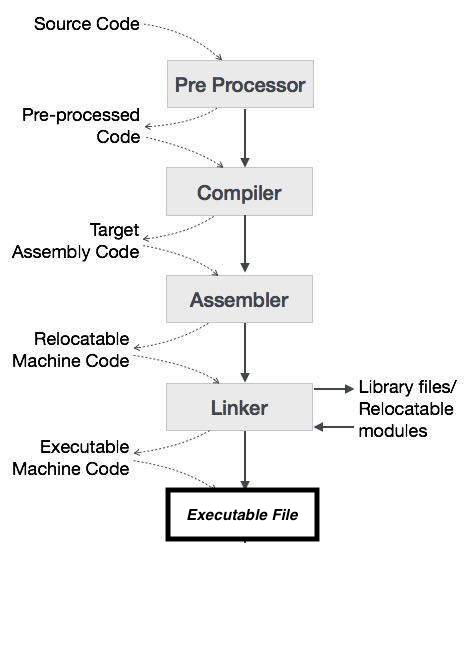
\includegraphics[width=0.5\linewidth]{c.png}
    \caption{C Code Compilation Steps}
\end{figure}

\subsubsection*{C++ Compiler Steps}
Example: Compilation of a C++ program to implement a simple class.

\begin{lstlisting}
#include <iostream>

class Rectangle {
private:
    double width;
    double height;

public:
    Rectangle(double w, double h) : width(w), height(h) {}

    double area() {
        return width * height;
    }
};

int main() {
    Rectangle rect(5.0, 3.0);
    std::cout << "Area: " << rect.area() << std::endl;
    return 0;
}
\end{lstlisting}

\paragraph*{Step 1: Preprocessing}
The preprocessor handles \#include directives, such as including the <iostream> header file. It also expands macros and resolves conditional compilation directives.

\paragraph*{Step 2: Compilation}
The C++ compiler performs lexical analysis, syntax analysis, and semantic analysis similar to the C compilation process. Additionally, it handles C++-specific features like classes, templates, and exception handling.

\paragraph*{Step 3: Code Generation}
The compiler generates assembly code from the AST. It applies optimizations specific to C++ such as function inlining, virtual function table generation, and name mangling.

\paragraph*{Step 4: Assembling}
The assembler converts the assembly code into object code, which contains machine instructions specific to the target architecture.

\paragraph*{Step 5: Linking}
The linker combines the object code with any necessary C++ libraries (such as the C++ Standard Library) and resolves external references. It creates an executable file that can be run on the target machine.

\begin{figure}[H]
    \centering
    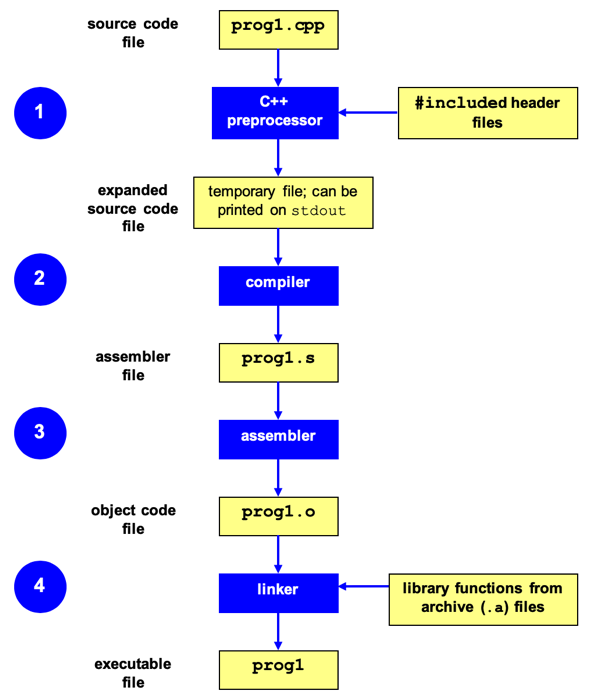
\includegraphics[width=0.5\linewidth]{c++.png}
    \caption{C++ Code Compilation Steps}
\end{figure}

\subsubsection*{Java Compiler Steps}
Example: Compilation of a Java program to implement a simple inheritance hierarchy.

\begin{lstlisting}
class Animal {
    public void makeSound() {
        System.out.println("Animal makes a sound");
    }
}

class Dog extends Animal {
    @Override
    public void makeSound() {
        System.out.println("Dog barks");
    }
}

public class Main {
    public static void main(String[] args) {
        Animal animal = new Animal();
        Dog dog = new Dog();

        animal.makeSound();
        dog.makeSound();
    }
}
\end{lstlisting}

\paragraph*{Step 1: Compilation}
The Java compiler (javac) compiles the Java source code into bytecode. It performs lexical analysis, syntax analysis, and semantic analysis. The compiler generates a .class file for each class in the program.

\paragraph*{Step 2: Class Loading}
The Java ClassLoader loads the bytecode of the required classes into the Java Virtual Machine (JVM). It locates and reads the .class files.

\paragraph*{Step 3: Bytecode Verification}
The JVM verifies the bytecode to ensure it is valid and does not violate any security restrictions. This step helps maintain the integrity and security of the Java runtime environment.

\paragraph*{Step 4: Execution}
The JVM interprets the bytecode and executes the program. It translates the bytecode into machine instructions specific to the target platform. The JVM also performs runtime optimizations using its Just-In-Time (JIT) compiler.

\begin{figure}[H]
    \centering
    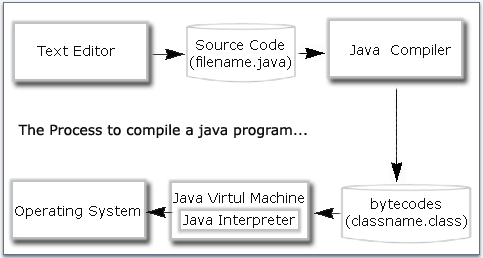
\includegraphics[width=0.7\linewidth]{java.png}
    \caption{Java Code Compilation Steps}
\end{figure}

\subsection*{Conclusion}
\addcontentsline{toc}{subsection}{Conclusion}
This case study explored the compilation process of C, C++, and Java programs. We analyzed the steps involved in each language's compilation process, including preprocessing, lexical analysis, syntax analysis, semantic analysis, code generation, and linking.

C and C++ follow a similar compilation process, with the addition of C++-specific features in the C++ compiler. The source code is preprocessed, compiled into assembly code, assembled into object code, and finally linked with libraries to create an executable.

Java, on the other hand, follows a different compilation process. The Java source code is compiled into bytecode, which is then executed by the Java Virtual Machine (JVM). The JVM performs class loading, bytecode verification, and execution, providing platform independence and enhanced security.

Understanding the compilation process of different programming languages is crucial for developers to write efficient and optimized code. It also helps in debugging and troubleshooting issues that may arise during the compilation and execution of programs.

\subsection*{References}
\addcontentsline{toc}{subsection}{References}
\begin{itemize}
    \item Aho, A. V., Lam, M. S., Sethi, R., \& Ullman, J. D. (2006). Compilers: Principles, Techniques, and Tools (2nd Edition). Addison-Wesley.
    \item Gosling, J., Joy, B., Steele, G., Bracha, G., \& Buckley, A. (2015). The Java Language Specification, Java SE 8 Edition. Oracle.
    \item Stroustrup, B. (2013). The C++ Programming Language (4th Edition). Addison-Wesley.
\end{itemize}

\subsection*{Experiment Steps}
\addcontentsline{toc}{subsection}{Experiment Steps}

\subsubsection*{Step 1: Setup the Development Environment}
Install the necessary compilers and development tools for C, C++, and Java on your system. This may include:
\begin{itemize}
    \item C Compiler (e.g., GCC)
    \item C++ Compiler (e.g., G++)
    \item Java Development Kit (JDK)
    \item Integrated Development Environment (IDE) or text editor of your choice
\end{itemize}

\subsubsection*{Step 2: Write Sample Programs}
Create sample programs in C, C++, and Java that demonstrate various language features and concepts. These programs should cover different aspects of the language, such as:
\begin{itemize}
    \item Basic input/output operations
    \item Control structures (if-else, loops)
    \item Functions or methods
    \item Arrays and data structures
    \item Object-oriented programming concepts (classes, inheritance, polymorphism)
\end{itemize}

\subsubsection*{Step 3: Compile the Programs}
Compile the sample programs using the respective compilers for each language. Observe the compilation process and note any warnings or errors generated by the compiler. Analyze the generated assembly code or bytecode to understand how the high-level code is translated into lower-level instructions.

\subsubsection*{Step 4: Execute the Programs}
Run the compiled programs and verify their output. Test various inputs and edge cases to ensure the programs behave as expected. Observe the runtime behavior and performance of the programs.

\subsubsection*{Step 5: Analyze the Compilation Process}
Study the different stages of the compilation process for each language. Use debugging tools or compiler flags to generate intermediate files (e.g., preprocessed code, assembly code) at each stage. Analyze these files to understand how the code is transformed and optimized during compilation.

\subsubsection*{Step 6: Compare and Contrast}
Compare the compilation process of C, C++, and Java. Identify the similarities and differences between them. Consider factors such as compilation time, memory usage, platform dependence, and runtime performance. Discuss the advantages and limitations of each language's compilation approach.

\subsubsection*{Step 7: Document and Present Findings}
Document your observations, analysis, and conclusions from the experiment. Prepare a report or presentation summarizing your findings. Include code snippets, compiler output, and performance metrics to support your analysis. Present your findings to your peers or instructor for discussion and feedback.

\subsection*{Evaluation}
\addcontentsline{toc}{subsection}{Evaluation}
The case study can be evaluated based on the following criteria:
\begin{itemize}
    \item Correctness and completeness of the sample programs
    \item Understanding of the compilation process for each language
    \item Depth of analysis and comparison between the languages
    \item Clarity and organization of the documentation and presentation
    \item Ability to answer questions and provide insights during the discussion
\end{itemize}

\subsection*{Limitations and Future Work}
\addcontentsline{toc}{subsection}{Limitations and Future Work}
This case study provides an overview of the compilation process for C, C++, and Java. However, it has some limitations:
\begin{itemize}
    \item The sample programs used in the experiment may not cover all the features and complexities of each language.
    \item The analysis is based on a specific set of compilers and tools, and the results may vary with different versions or implementations.
    \item The case study does not delve into advanced topics such as compiler optimizations, linker scripts, or runtime environments.
\end{itemize}

Future work can include:
\begin{itemize}
    \item Exploring additional programming languages and their compilation processes
    \item Investigating advanced compiler optimizations and their impact on performance
    \item Analyzing the role of linkers and runtime environments in the overall execution of programs
    \item Examining the compilation process for domain-specific languages or scripting languages
\end{itemize}

\subsection*{Acknowledgments}
\addcontentsline{toc}{subsection}{Acknowledgments}
We would like to acknowledge the contributions of the following individuals and resources in the preparation of this case study:
\begin{itemize}
    \item The developers and maintainers of the GCC, G++, and Java compilers for their excellent tools and documentation.
    \item The authors of the referenced books and articles for their valuable insights and explanations of compiler concepts.
    \item The open-source community for providing access to a wide range of programming resources and examples.
\end{itemize}

\subsection*{Glossary}
\addcontentsline{toc}{subsection}{Glossary}
\begin{description}
    \item[Assembly Code] Low-level code that represents machine instructions and is specific to a particular processor architecture.
    \item[Bytecode] Intermediate code generated by compilers for languages like Java. It is executed by a virtual machine.
    \item[Compiler] A program that translates high-level source code into lower-level code, such as assembly code or machine code.
    \item[Interpreter] A program that directly executes high-level source code without prior compilation.
    \item[Lexical Analysis] The process of breaking down the source code into a sequence of tokens, such as keywords, identifiers, and literals.
    \item[Linker] A program that combines object files and resolves external references to create an executable file.
    \item[Object Code] Machine code that is generated by the assembler from the assembly code.
    \item[Preprocessor] A program that processes directives and macros in the source code before the actual compilation begins.
    \item[Semantic Analysis] The process of checking the source code for semantic errors and verifying type consistency.
    \item[Syntax Analysis] The process of checking the source code against the grammar rules of the programming language.
\end{description}


%------------------ EXP 2 Page ------------------
\newpage
\section*{Experiment 2: Lexical Analyzer : Token Counter + Data Types Identification}
\addcontentsline{toc}{section}{Experiment 2: Lexical Analyzer : Token Counter + Data Types Identification}

\subsection*{Aim}
\addcontentsline{toc}{subsection}{Aim}
The aim of this experiment is to design and implement a simple lexical analyzer in C++ that counts tokens and identifies data types within a given expression.

\subsection*{Objectives}
\addcontentsline{toc}{subsection}{Objectives}
\begin{itemize}
    \item To understand the concept of lexical analysis in compiler design.
    \item To implement token counting logic in C++.
    \item To differentiate and identify various tokens such as operators, identifiers, separators, and literals.
    \item To familiarize with the process of recognizing data types within expressions.
\end{itemize}

\subsection*{Experiment Code}
\addcontentsline{toc}{subsection}{Experiment Code and Output}
\begin{lstlisting}
#include <iostream>
#include <string>
#include <cctype>
bool isOperator(char c)
{
   return c == '+' || c == '-' || c == '*' || c == '/';
}
bool isSeparator(char c)
{
   return c == ';' || c == ',' || c == '(' || c == ')';
}
int main()
{
   std::string expression;
   std::cout << "Enter the expression: ";
   std::getline(std::cin, expression);
   std::string token;
   int tokenCount = 0;
   bool inString = false;
   bool inComment = false;
   for (size_t i = 0; i < expression.length(); ++i)
   {
      char c = expression[i];
      if (inComment)
      {
         if (c == '*' && i + 1 < expression.length() && expression[i + 1] == '/')
         {
            // End of block comment
            inComment = false;
            i++; // Skip the closing '/'
         }
         continue; // Ignore everything inside comments
      }
      if (inString)
      {
         token += c;
         if (c == '"')
         {
            // End of string literal
            inString = false;
            std::cout << "'" << token << "' (string)\n";
            tokenCount++;
            token.clear();
         }
         continue;
      }
      if (c == '"')
      {
         if (!token.empty())
         {
            std::cout << "'" << token << "' (identifier)\n";
            tokenCount++;
            token.clear();
         }
         inString = true;
         token += c;
         continue;
      }
      if (isSeparator(c))
      {
         if (!token.empty())
         {
            std::cout << "'" << token << "' (identifier)\n";
            tokenCount++;
            token.clear();
         }
         std::cout << "'" << c << "' (separator)\n";
         tokenCount++; // Count separators
         continue;
      }
      if (isOperator(c))
      {
         if (!token.empty())
         {
            std::cout << "'" << token << "' (identifier)\n";
            tokenCount++;
            token.clear();
         }
         if (c == '+' && i + 1 < expression.length() && expression[i + 1] == '+')
         {
            std::cout << "'++' (increment operator)\n";
            i++; // Skip next character
         }
         else
         {
            std::cout << "'" << c << "' (operator)\n";
         }
         tokenCount++;
         continue;
      }
      if (c == '/' && i + 1 < expression.length() && expression[i + 1] == '*')
      {
         // Start of block comment
         inComment = true;
         i++; // Skip the opening '*'
         continue;
      }
      if (!std::isspace(c))
      {
         token += c;
      }
      else if (!token.empty())
      {
         std::cout << "'" << token << "' (identifier)\n";
         tokenCount++;
         token.clear();
      }
   }
   if (!token.empty())
   {
      std::cout << "'" << token << "' (identifier)\n";
      tokenCount++;
   }
   std::cout << "The number of tokens = " << tokenCount << std::endl;
   return 0;
}
\end{lstlisting}
\begin{figure}[H]
    \centering
    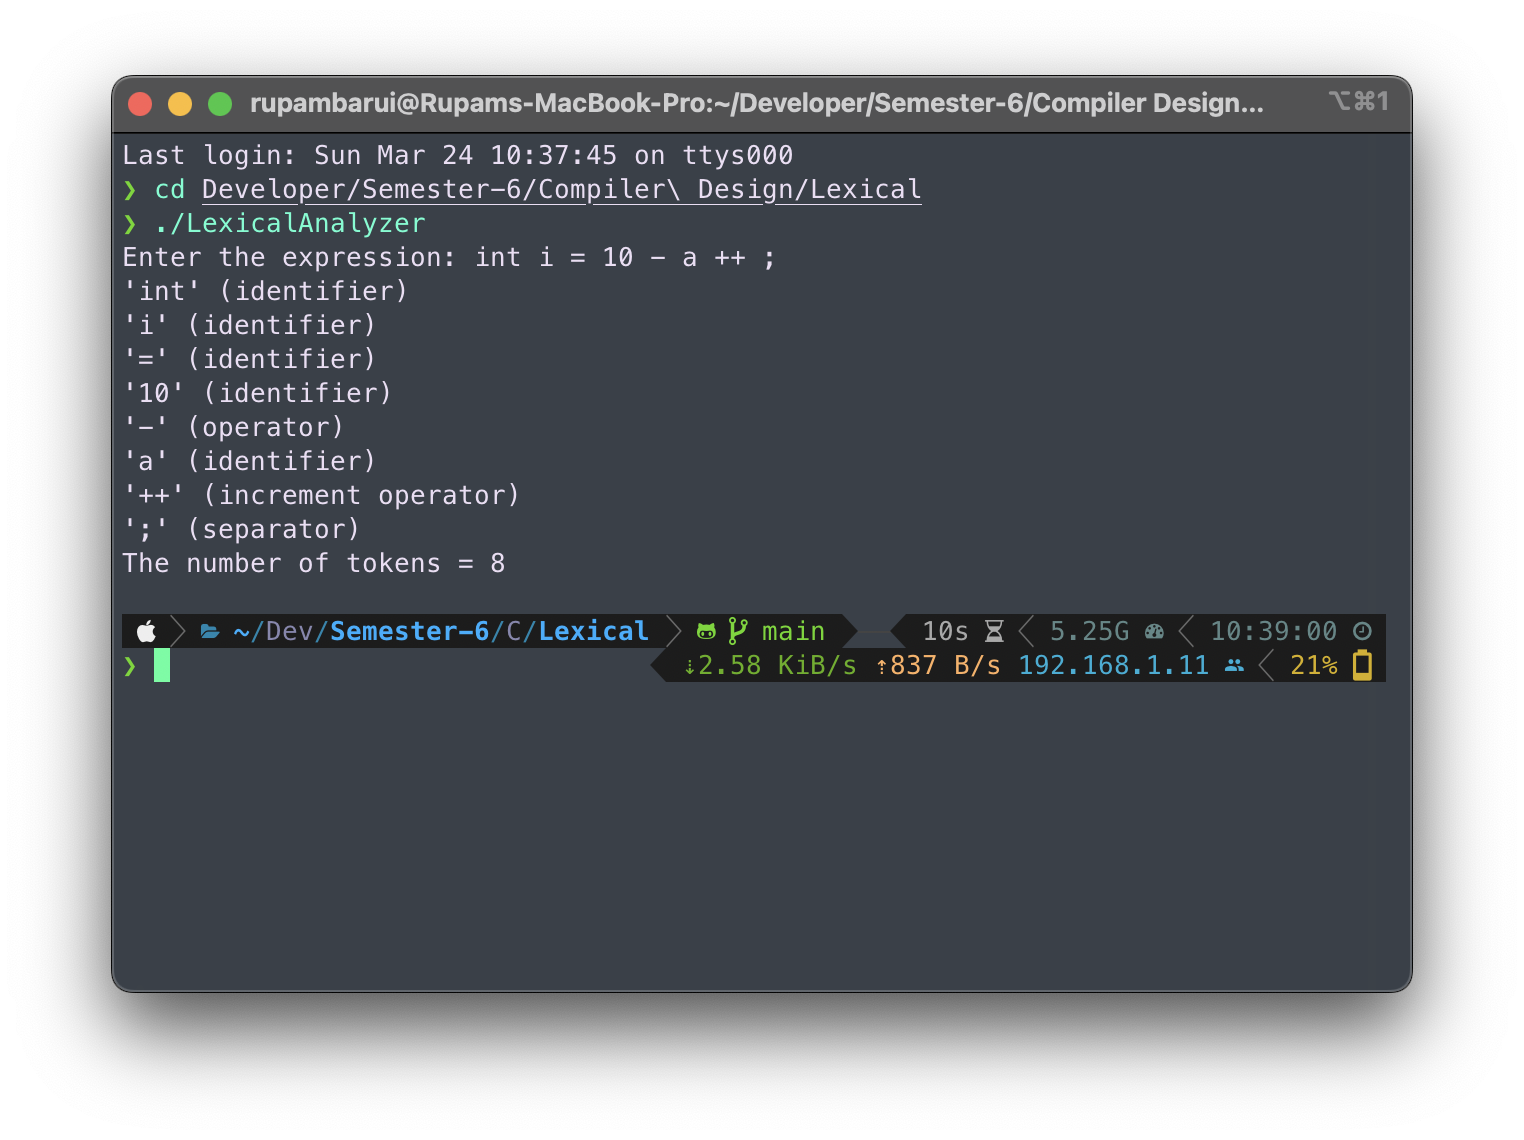
\includegraphics[width=1\linewidth]{exp2output.png}
    \caption{Lexical Analyser}
\end{figure}

%------------------ EXP 3 Page ------------------
\newpage
\section*{Experiment 3: Lex Program : Identify the strings ending with 11}
\addcontentsline{toc}{section}{Experiment 3: Lex Program : Identify the strings ending with 11}

\subsection*{Aim}
\addcontentsline{toc}{subsection}{Aim}
The aim of this experiment is to design and implement a lex program which can identify the strings passed as input which ends with 11.

\subsection*{Objectives}
\addcontentsline{toc}{subsection}{Objectives}
\begin{itemize}
    \item To understand the concept of regular expressions and their application in lexical analysis.
    \item To gain practical experience with the lex (or flex) tool for pattern matching.
    \item To implement a regular expression that matches strings ending with "11."
    \item To develop a lex program that can correctly identify and accept input strings that meet the specified pattern criteria.
    \item To test the lex program with various input cases to ensure accuracy and robustness.
\end{itemize}

\subsection*{Experiment Code}
\addcontentsline{toc}{subsection}{Experiment Code and Output}
\begin{lstlisting}
%{
#include <stdio.h>
int count_ending_with_11 = 0;
%}
%%
.*11\n { count_ending_with_11++;   printf("Found a line ending with '11': %s", yytext); }
.|\n   { /* Ignore all other characters */ }

%%

int main(int argc, char **argv) {
    yylex();
    printf("Total number of lines ending with '11': %d\n", count_ending_with_11);
    return 0;
}

int yywrap() {
    return 1;
}
\end{lstlisting}
\begin{figure}[H]
    \centering
    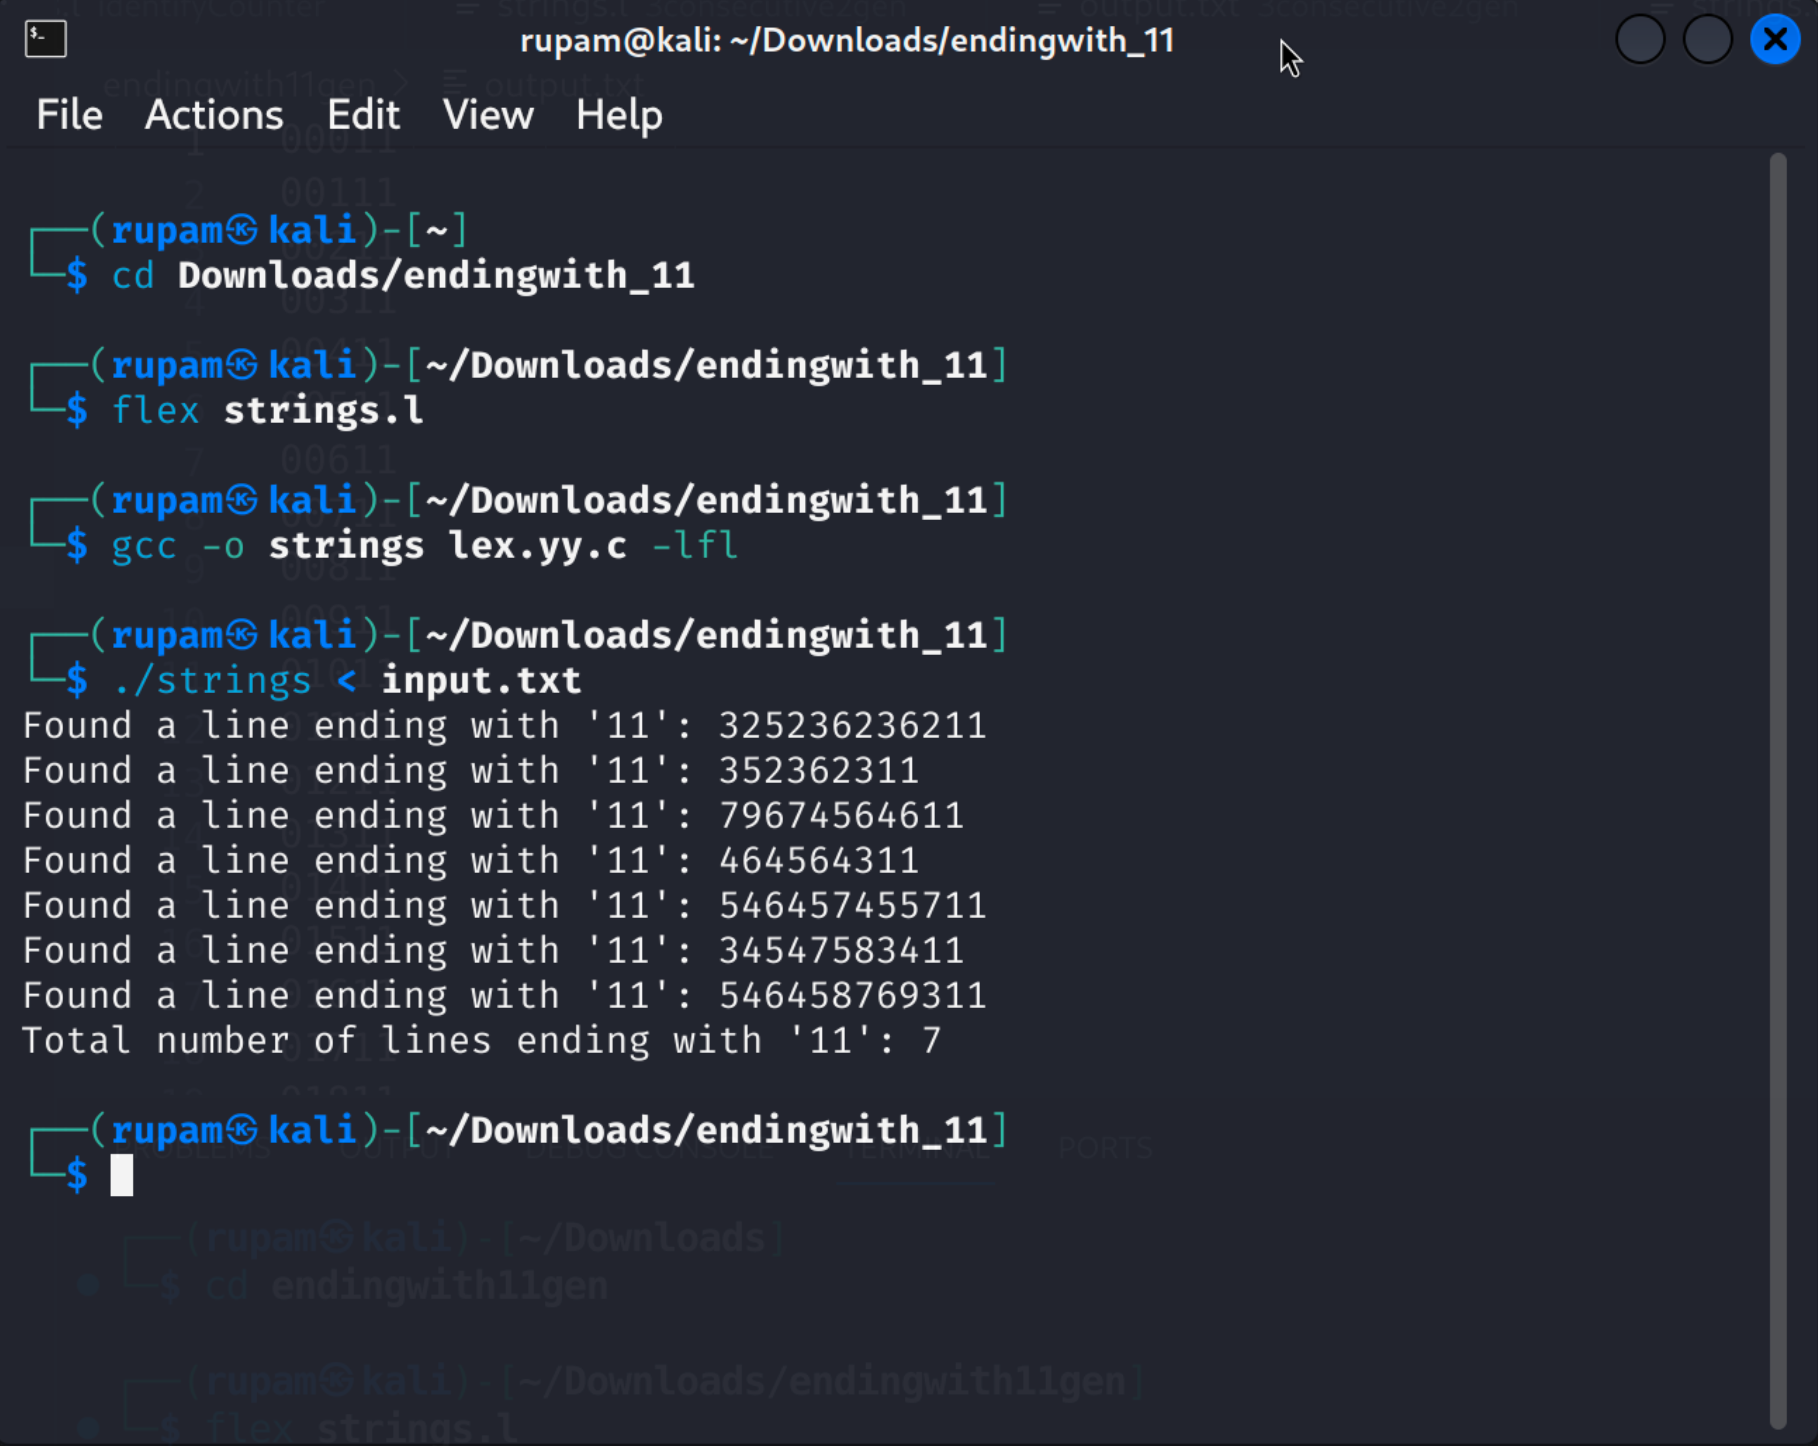
\includegraphics[width=1\linewidth]{exp3output.png}
    \caption{Strings ending with 11}
\end{figure}

%------------------ EXP 4 Page ------------------
\newpage
\section*{Experiment 4: Lex Program : Identify the strings with 3 consecutive 2s}
\addcontentsline{toc}{section}{Experiment 4: Lex Program : Identify the strings with 3 consecutive 2s}

\subsection*{Aim}
\addcontentsline{toc}{subsection}{Aim}
The aim of this experiment is to design and implement a lex program that can identify strings passed as input containing three consecutive '2's.

\subsection*{Objectives}
\addcontentsline{toc}{subsection}{Objectives}
\begin{itemize}
    \item To understand how to construct regular expressions for pattern matching specific string conditions.
    \item To gain practical experience with the lex (or flex) tool for creating lexical analyzers.
    \item To implement a regular expression that identifies strings containing "222."
    \item To develop a lex program that recognizes and flags input strings containing three consecutive '2's.
    \item To validate the functionality of the lex program through a series of test cases with various input strings.
\end{itemize}

\subsection*{Experiment Code}
\addcontentsline{toc}{subsection}{Experiment Code and Output}
\begin{lstlisting}
%{
#include <stdio.h>

int count_with_222 = 0;
%}
%%
.*222 { count_with_222++;   printf("\nFound a line with '222': %s", yytext); }
.|\n   { /* Ignore all other characters */ }
%%
int main(int argc, char **argv) {
    yylex();
    printf("\nTotal number of lines with '222': %d\n", count_with_222);
    return 0;
}

int yywrap() {
    return 1;
}
\end{lstlisting}
\begin{figure}[H]
    \centering
    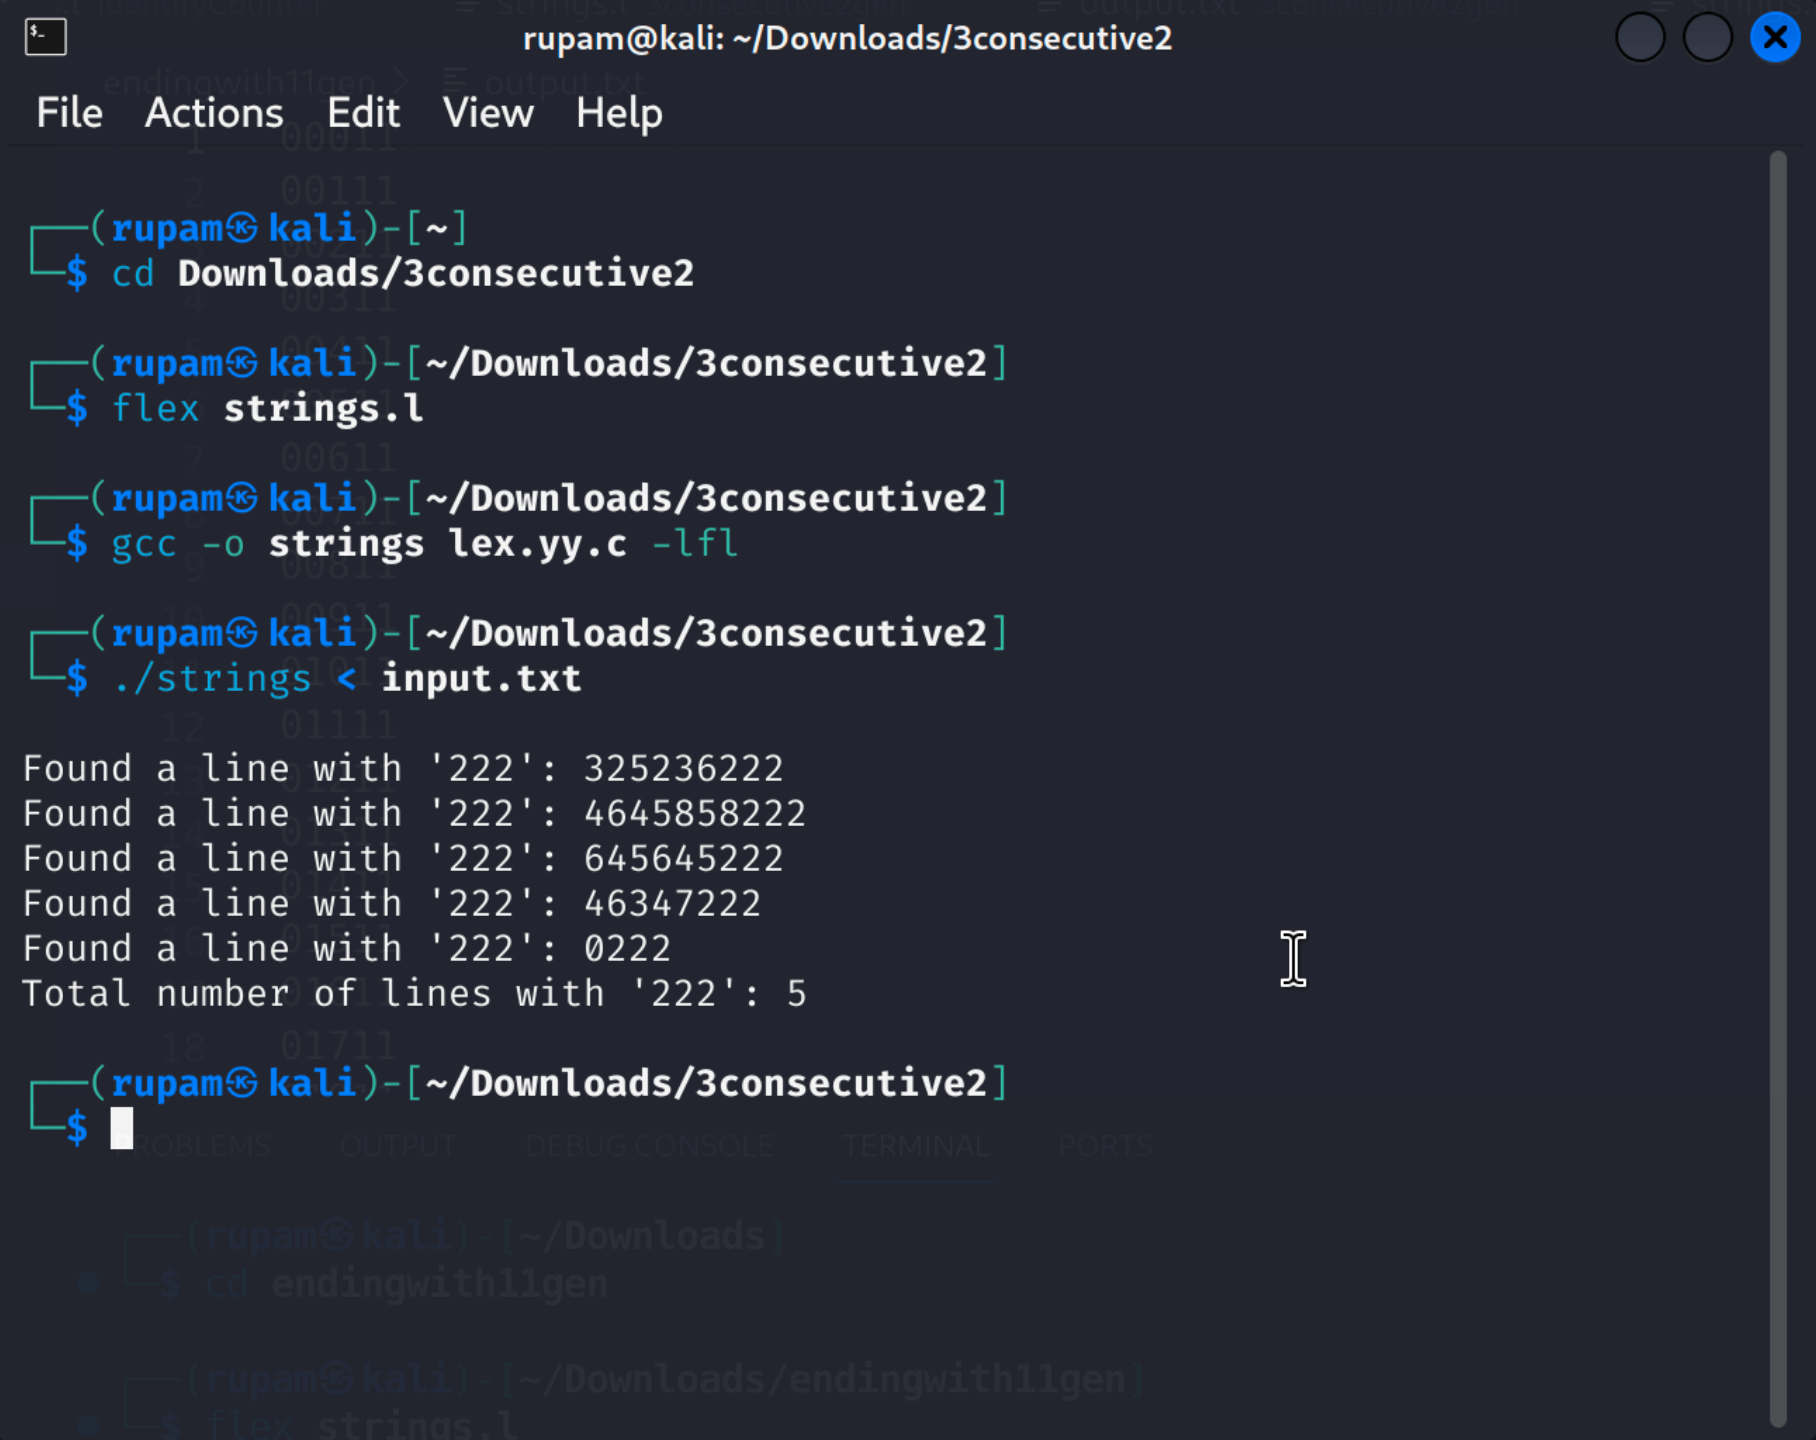
\includegraphics[width=1\linewidth]{exp4output.png}
    \caption{Srings Containing 3 consecutive 2s}
\end{figure}

%------------------ EXP 5 Page ------------------
\newpage
\section*{Experiment 5: Lex Program : Identify the strings such that the 10th symbol from right end is 1.}
\addcontentsline{toc}{section}{Experiment 5: Lex Program : Identify the strings such that the 10th symbol from right end is 1.}

\subsection*{Aim}
\addcontentsline{toc}{subsection}{Aim}
The aim of this experiment is to design and implement a lex program that can identify strings passed as input which have the 10th symbol from the right end as '1'.

\subsection*{Objectives}
\addcontentsline{toc}{subsection}{Objectives}
\begin{itemize}
    \item To understand the intricacies of pattern matching and regular expressions for positions within strings.
    \item To explore the lex (or flex) tool capabilities for developing lexical analyzers with position-dependent patterns.
    \item To design a regular expression that can precisely match strings with the 10th symbol from the right end being '1'.
    \item To create a lex program capable of processing input strings and correctly identifying those that match the specified positional pattern.
    \item To conduct thorough testing of the lex program against a variety of input cases to confirm its functionality and reliability.
\end{itemize}

\subsection*{Experiment Code}
\addcontentsline{toc}{subsection}{Experiment Code and Output}
\begin{lstlisting}
%{
#include <stdio.h>
int count_10th_from_right_is_1 = 0;
%}
%%
.*1.{9} { count_10th_from_right_is_1++;   printf("Found a line with '1' as 10th character from the right: %s", yytext); }
.|\n      { /* Ignore all other characters */ }
%%
int main(int argc, char **argv) {
    yylex();
    printf("\nTotal number of lines where the 10th character from the right is '1': %d\n", count_10th_from_right_is_1);
    return 0;
}

int yywrap() {
    return 1;
}
\end{lstlisting}
\begin{figure}[H]
    \centering
    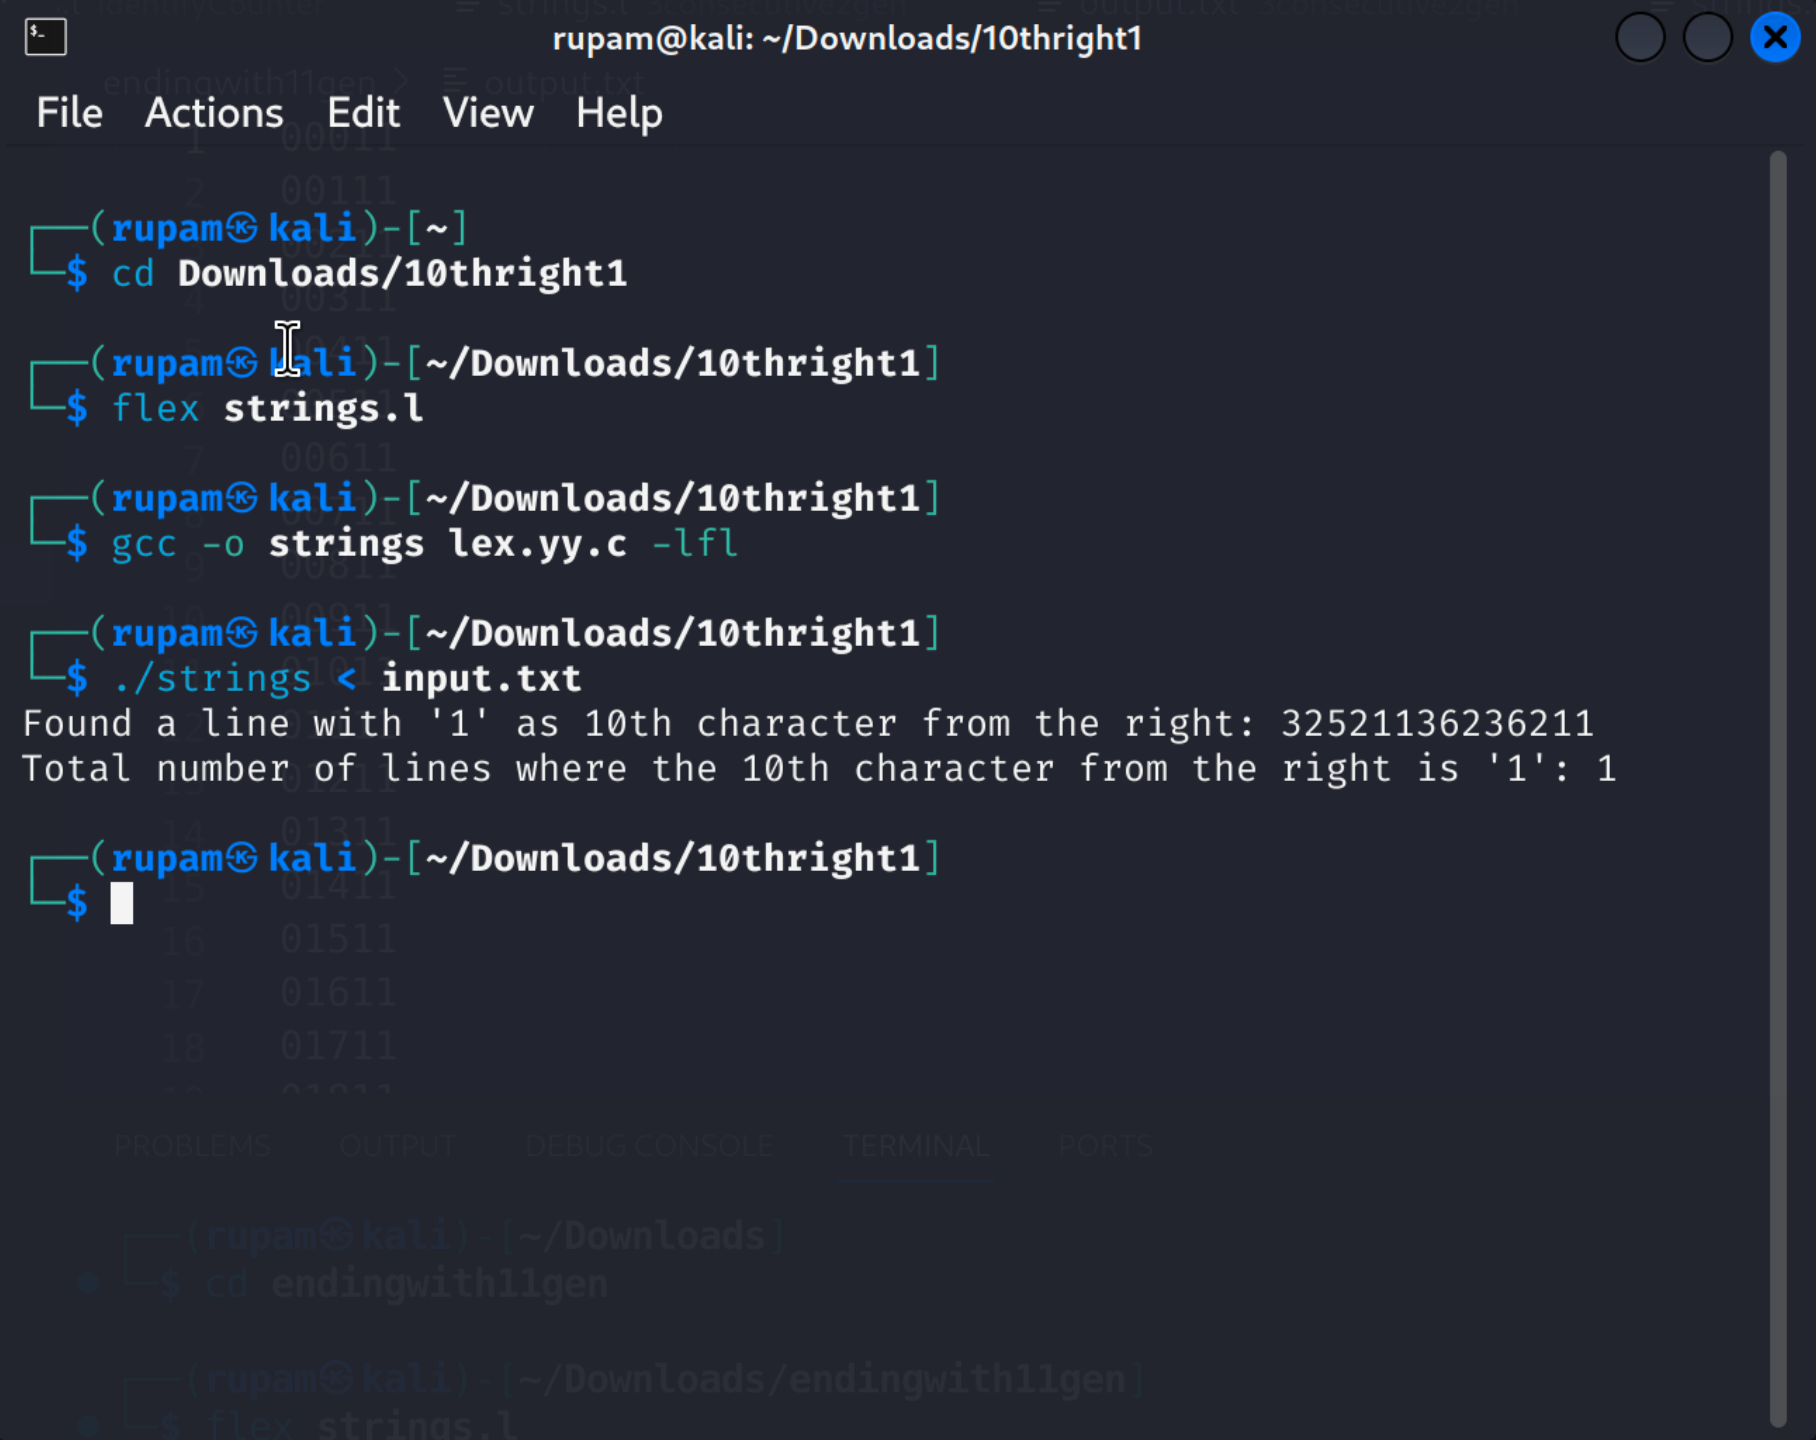
\includegraphics[width=1\linewidth]{exp5output.png}
    \caption{Enter Caption}
\end{figure}

%------------------ EXP 6 Page ------------------
\newpage
\section*{Experiment 6: Lex Program : Identify all the 4 digit numbers whose sum is 9.}
\addcontentsline{toc}{section}{Experiment 6: Lex Program : Identify all the 4 digit numbers whose sum is 9.}

\subsection*{Aim}
\addcontentsline{toc}{subsection}{Aim}
The aim of this experiment is to design and implement a lex program to identify all 4-digit numbers inputted by the user whose digits sum to 9.

\subsection*{Objectives}
\addcontentsline{toc}{subsection}{Objectives}
\begin{itemize}
    \item To understand and apply regular expressions to match specific numeric patterns.
    \item To gain experience with lex (or flex) to create lexical analyzers focused on number processing.
    \item To implement a regular expression that matches 4-digit numbers with a digit sum of 9.
    \item To develop a lex program that accurately sorts through user input and identifies valid 4-digit numbers based on the sum of their digits.
    \item To test the lex program thoroughly with a variety of input numbers to ensure correct identification and functionality.
\end{itemize}

\subsection*{Experiment Code}
\addcontentsline{toc}{subsection}{Experiment Code and Output}
\begin{lstlisting}
%{
#include <stdio.h>
int sum_of_digits(const char *str);
int count_sum_9 = 0;

%}

%%
[0-9]{4}  { if (sum_of_digits(yytext) == 9) {count_sum_9++ ; printf("Valid number: %s\n", yytext);}}
.|\n       { /* ignore other input */ }
%%

int sum_of_digits(const char *str) {
    int sum = 0;
    while(*str) {
        sum += *str - '0'; // Convert char digit to int and add to sum
        str++;
    }
    return sum;
}

int yywrap() { return 1; }

int main() {
    yylex();
    printf("Total number of strings whose digits add up to 9 : %d\n", count_sum_9);
    return 0;
}
\end{lstlisting}
\begin{figure}[H]
    \centering
    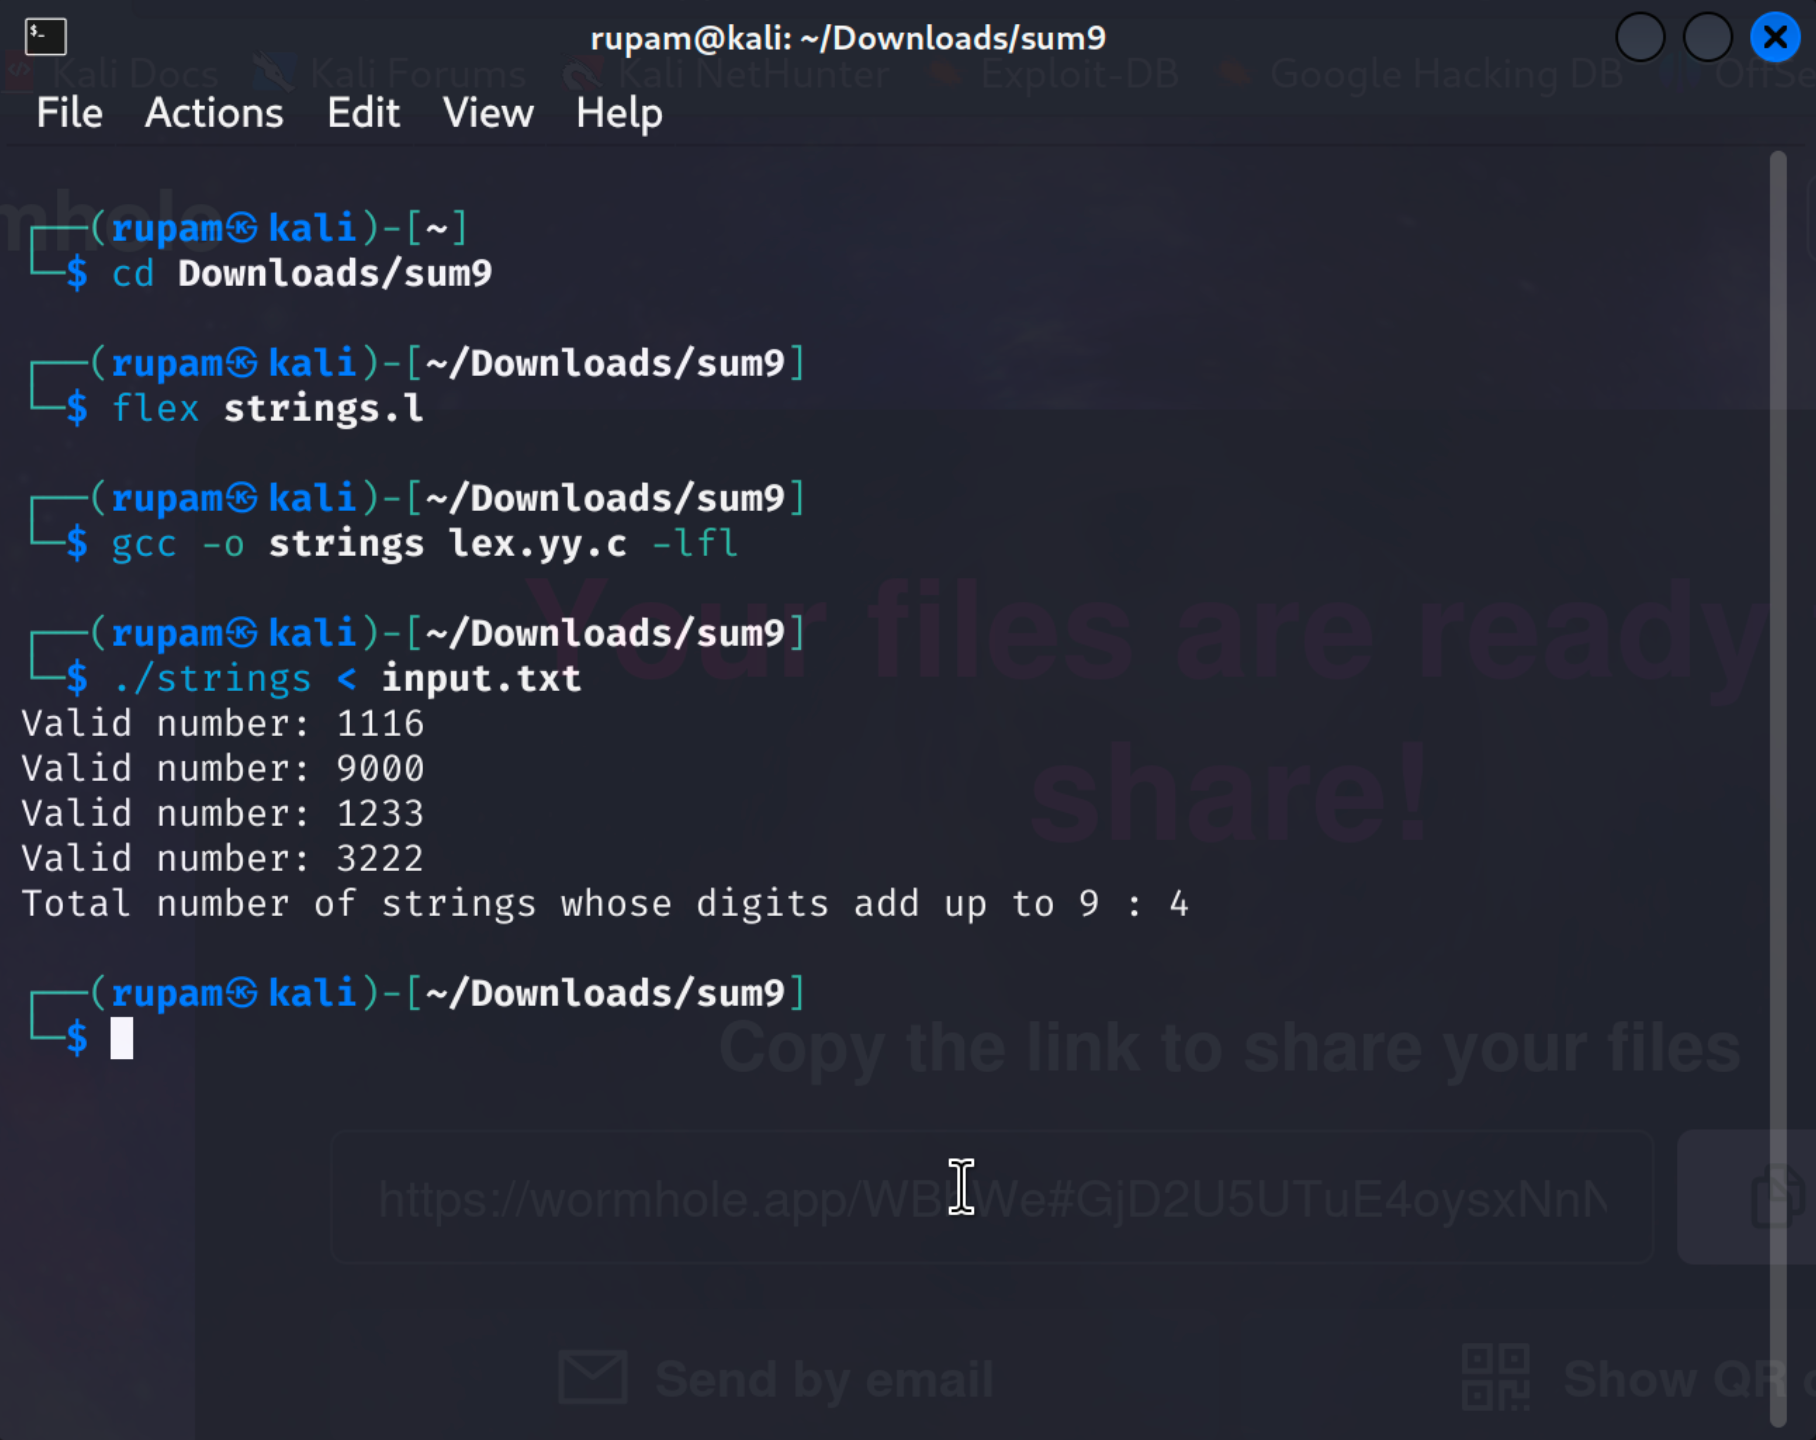
\includegraphics[width=1\linewidth]{exp6output.png}
    \caption{Digits with sum of 9}
\end{figure}

%------------------ EXP 7 Page ------------------
\newpage
\section*{Experiment 7: Lex Program : Identify the set of all 4 digit numbers whose individual digits are in ascending order from left to right.}
\addcontentsline{toc}{section}{Experiment 7: Lex Program : Identify the set of all 4 digit numbers whose individual digits are in ascending order from left to right.}

\subsection*{Aim}
\addcontentsline{toc}{subsection}{Aim}
The aim of this experiment is to design and implement a lex program to identify all 4-digit numbers inputted by the user whose digits are in strictly ascending order from left to right.

\subsection*{Objectives}
\addcontentsline{toc}{subsection}{Objectives}
\begin{itemize}
    \item To understand and construct regular expressions that capture numeric patterns with ordered sequences.
    \item To gain practical experience with lex (or flex) for developing lexical analyzers that can process and recognize ordered patterns in numbers.
    \item To devise a lex program that identifies 4-digit numbers with digits in ascending order, ensuring that each digit is less than the digit to its right.
    \item To develop the capability within the lex program to filter user input and exclusively identify and report numbers that adhere to the ascending order condition.
    \item To perform comprehensive testing of the lex program with diverse input cases to verify its accuracy and robustness.
\end{itemize}

\subsection*{Experiment Code}
\addcontentsline{toc}{subsection}{Experiment Code and Output}
\begin{lstlisting}
%{
#include <stdio.h>

int count_ascending = 0;

int check_ascending(char *num) {
    for(int i = 0; i < 3; ++i) {
         if(num[i] >= num[i+1]) {
             return 0;
         }
    }
    return 1;
}

%}

%%

[0-9]{4}   { if (check_ascending(yytext)) { count_ascending++; printf("Found an ascending number: %s\n", yytext); } }
.|\n { /* Ignore all other characters */ }

%%

int main(int argc, char **argv) {
    yylex();
    printf("Total number of ascending 4 digit numbers: %d\n", count_ascending);
    return 0;
}

int yywrap() {
    return 1;
}
\end{lstlisting}
\begin{figure}[H]
    \centering
    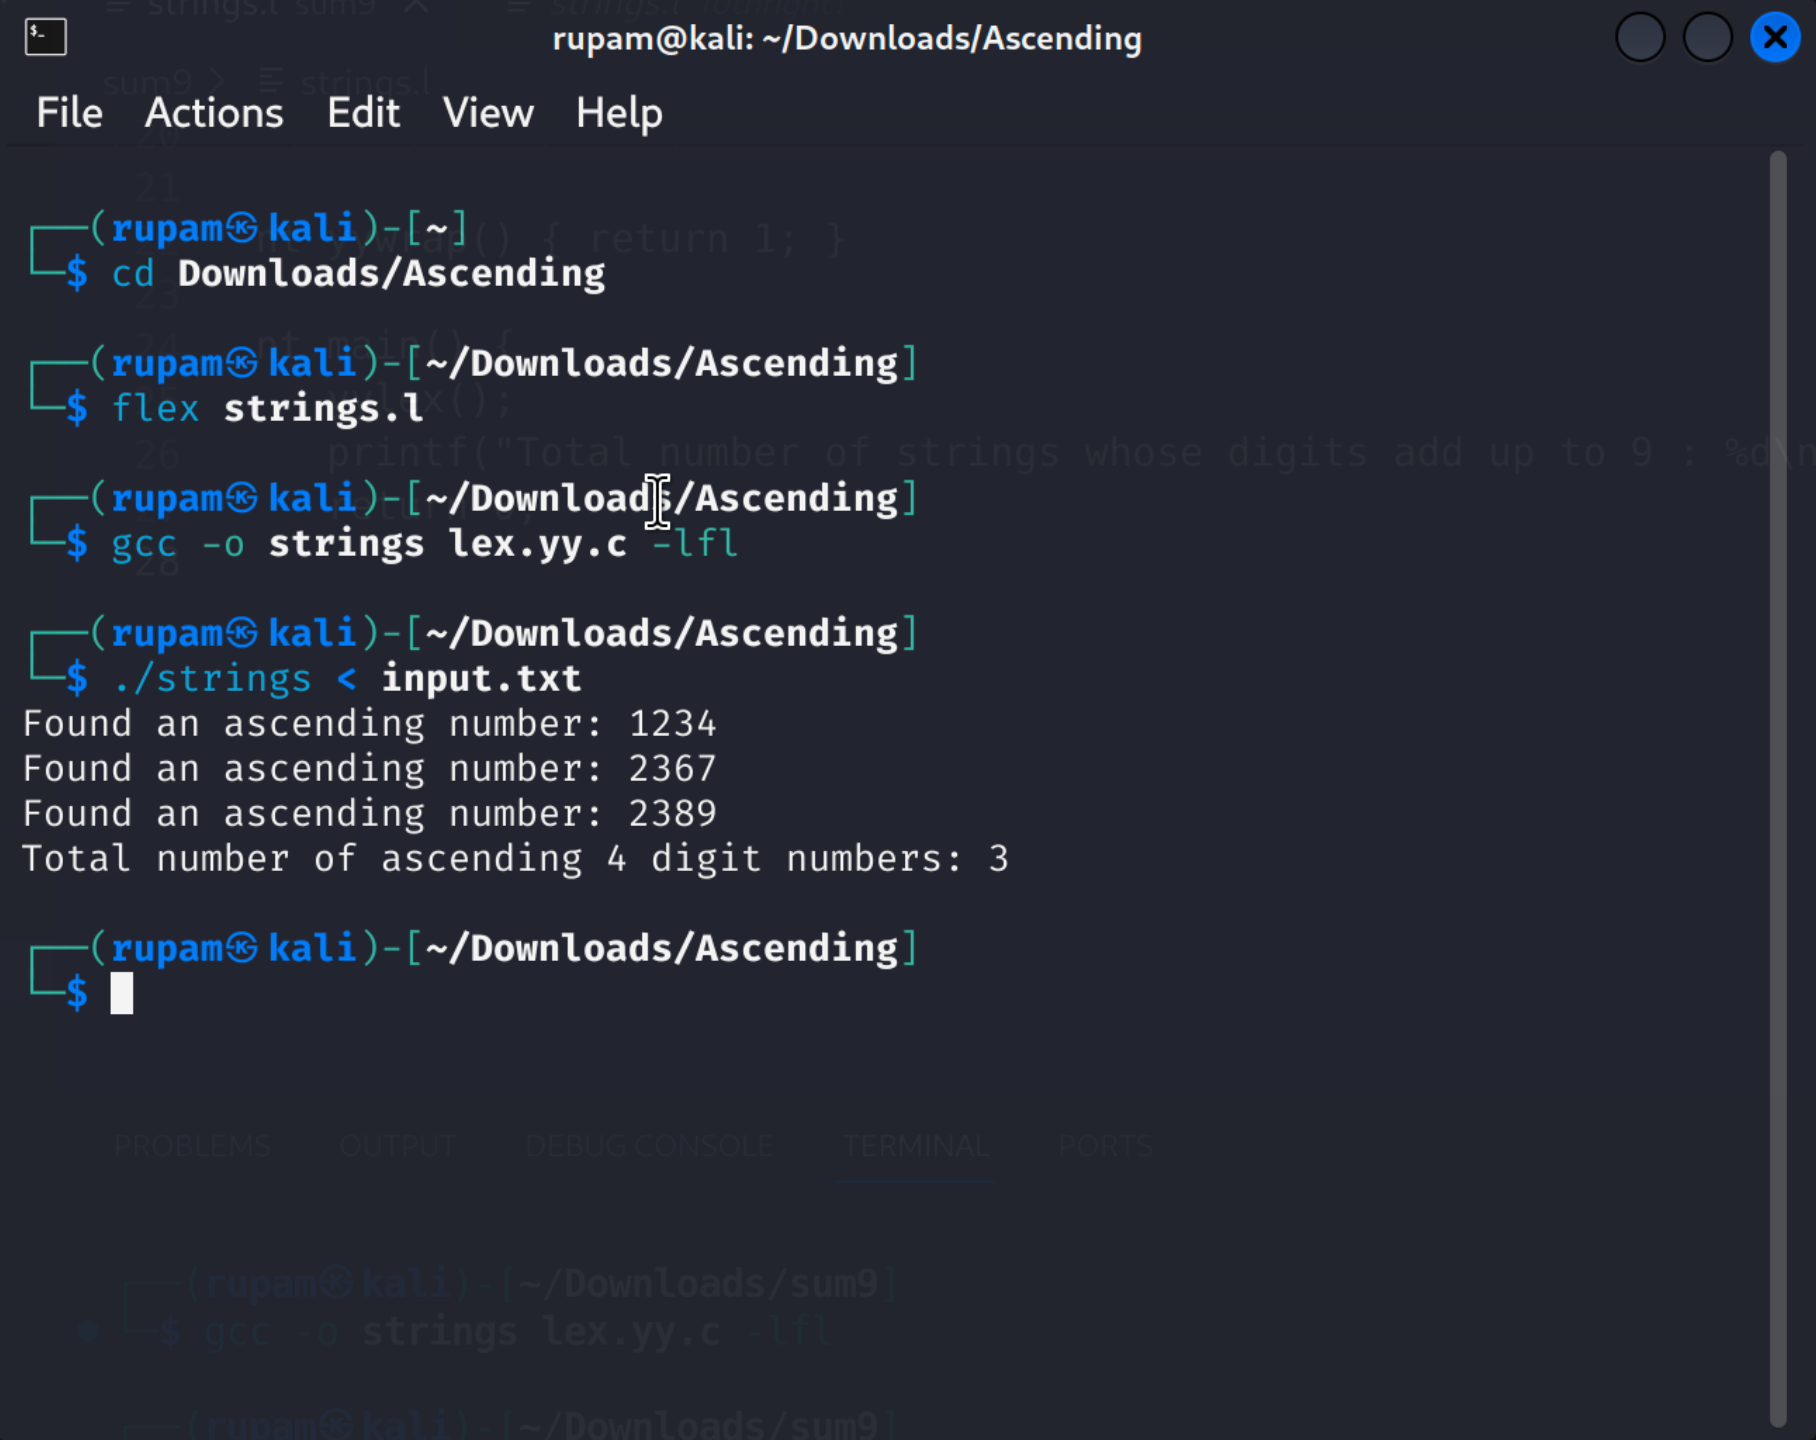
\includegraphics[width=1\linewidth]{exp7output.png}
    \caption{numbers containing the digits in ascending order}
\end{figure}

%------------------ EXP 8 Page ------------------
\newpage
\section*{Experiment 8: Lex Program : Identify all the set of all floating point numbers.}
\addcontentsline{toc}{section}{Experiment 8: Lex Program : Identify all the set of all Floating point numbers.}

\subsection*{Aim}
\addcontentsline{toc}{subsection}{Aim}
The aim of this experiment is to design and implement a lex program that can identify all floating point numbers from user input.

\subsection*{Objectives}
\addcontentsline{toc}{subsection}{Objectives}
\begin{itemize}
    \item To understand the usage and development of regular expressions for recognizing floating point numerical patterns.
    \item To gain practical experience with lex (or flex) for creating lexical analyzers that identify different representations of floating point numbers.
    \item To develop a lex program that effectively matches and identifies floating point numbers which can have a fractional part, an integer part, and possibly an exponent part.
    \item To design the lex program to accurately analyze a stream of user input and catalog all instances of floating point numbers.
    \item To thoroughly verify the accuracy and reliability of the lex program by testing it with diverse, real-world-like input cases, including challenging edge cases.
\end{itemize}

\subsection*{Experiment Code}
\addcontentsline{toc}{subsection}{Experiment Code and Output}
\begin{lstlisting}
%{
#include <stdio.h>
int count = 0;
%}

digit       [0-9]
opt_sign    [-+]?
exp_part    ([eE]{opt_sign}{digit}+)
number      ({opt_sign}{digit}*"."{digit}+{exp_part}?)|({opt_sign}{digit}+"."{digit}*{exp_part}?)

%%
{number} { count++; printf("Found floating-point number: %s\n", yytext); }
%%

int main(int argc, char **argv) {
    yylex();
    printf("\nTotal number of floating-point numbers found: %d\n", count);
    return 0;
}

int yywrap(void) {
    return 1;
}
\end{lstlisting}
\begin{figure}[H]
    \centering
    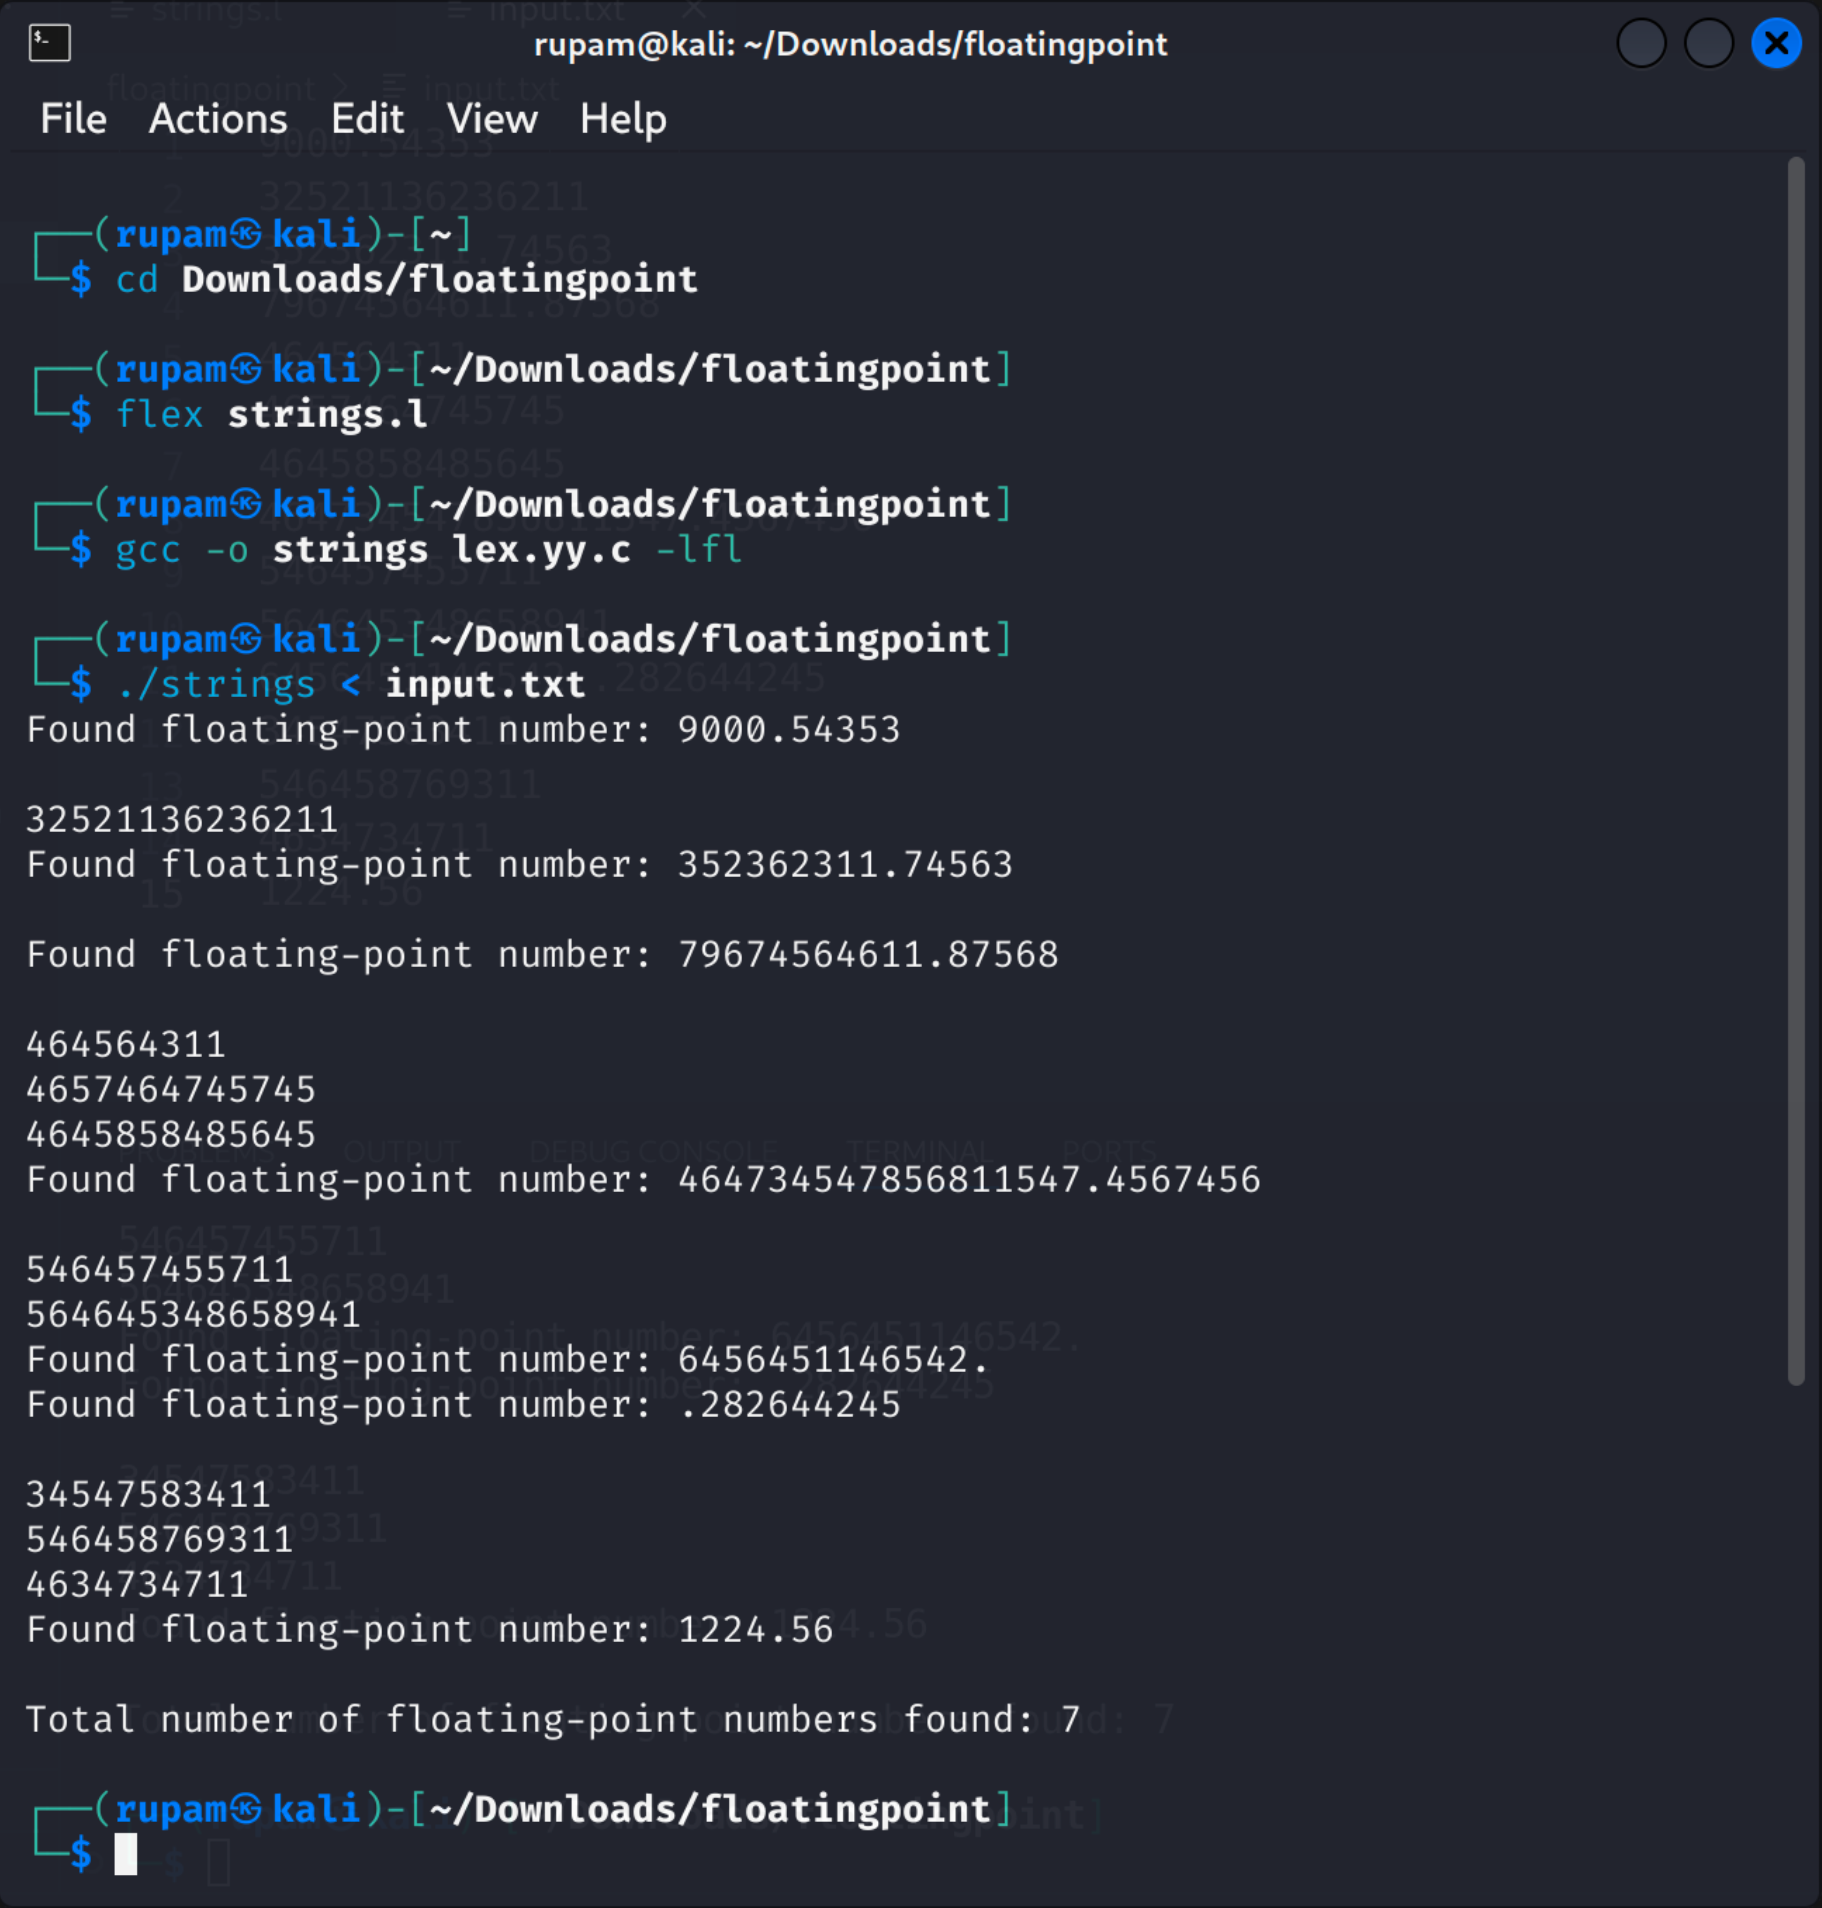
\includegraphics[width=1\linewidth]{exp8output.png}
    \caption{Floating Point numbers}  
\end{figure}

%------------------ EXP 9 Page ------------------
\newpage
\section*{Experiment 9: Lex Program : Count the number of words in a text file.}
\addcontentsline{toc}{section}{Experiment 9: Lex Program : Count the number of words in a text file.}

\subsection*{Aim}
\addcontentsline{toc}{subsection}{Aim}
The aim of this experiment is to design and implement a lex program that counts the number of words in a given text file.

\subsection*{Objectives}
\addcontentsline{toc}{subsection}{Objectives}
\begin{itemize}
    \item To become familiar with the lex (or flex) utility for lexical analysis in text processing.
    \item To understand and apply regular expressions to identify word boundaries.
    \item To create a lex program that counts words by recognizing sequences of characters separated by whitespace or punctuation.
    \item To process a text file and efficiently determine the total number of words it contains.
    \item To test the program's accuracy and reliability by analyzing text files with varying content and structure.
\end{itemize}

\subsection*{Experiment Code}
\addcontentsline{toc}{subsection}{Experiment Code and Output}
\begin{lstlisting}
%{
int word_count = 0;
%}

%%

[a-zA-Z]+   { word_count++; }

\n          { /* you can count lines here if you want to */ }

.           { /* ignore other characters */ }

%%

int main(int argc, char **argv) {
    yylex();
    printf("The number of words is: %d\n", word_count);
    return 0;
}

int yywrap(void) {
    return 1; // Returning 1 indicates that there's no more input
}
\end{lstlisting}
\begin{figure}[H]
    \centering
    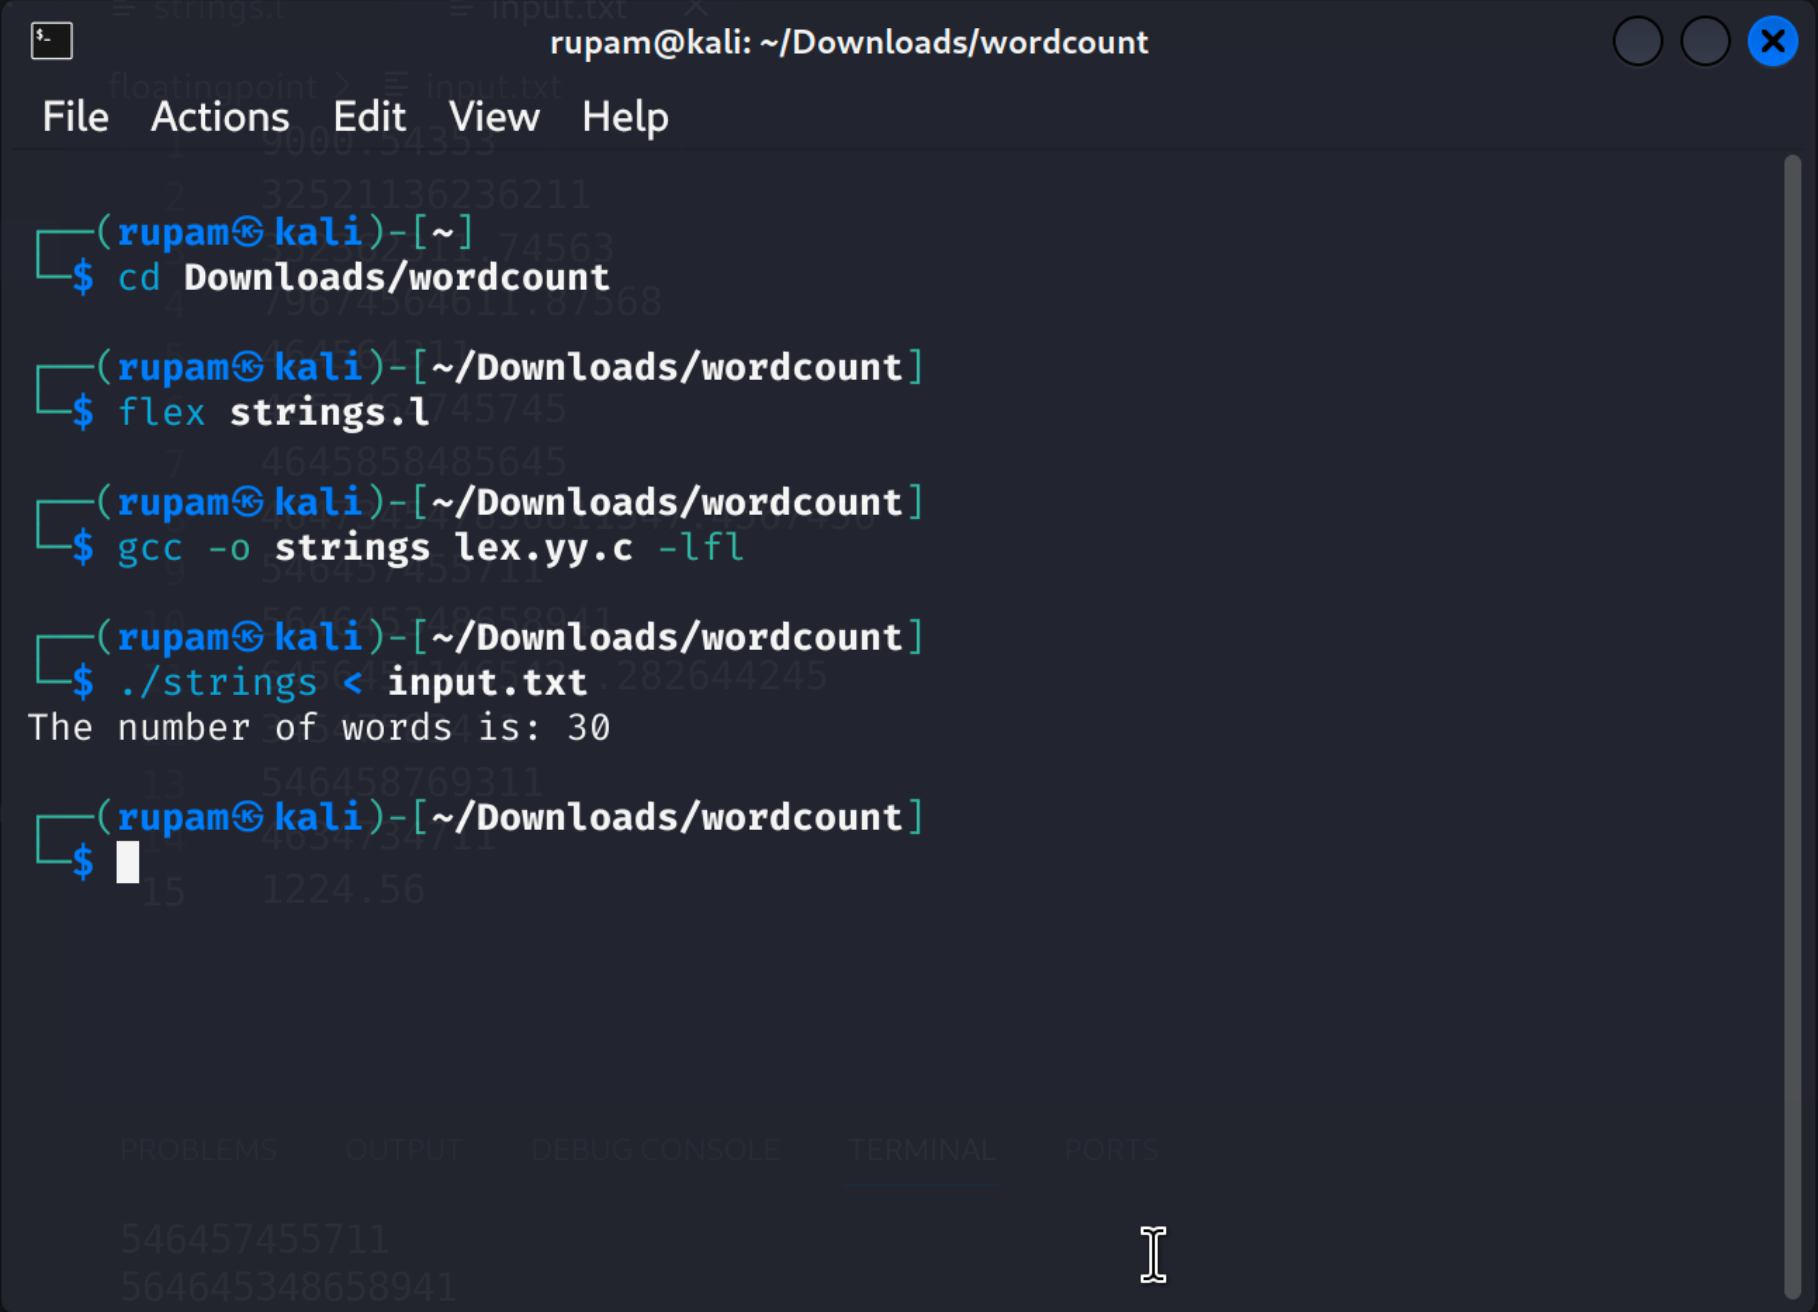
\includegraphics[width=1\linewidth]{exp9output.png}
    \caption{Enter Caption}
\end{figure}

%------------------ EXP 10 Page ------------------
\newpage
\section*{Experiment 10: Lex Program : Identify keywords and convert it into upper-case.}
\addcontentsline{toc}{section}{Experiment 10: Lex Program : Identify keywords and convert it into upper-case.}

\subsection*{Aim}
\addcontentsline{toc}{subsection}{Aim}
The aim of this experiment is to design and implement a lex program that identifies programming language keywords in the input and converts them into uppercase.

\subsection*{Objectives}
\addcontentsline{toc}{subsection}{Objectives}
\begin{itemize}
    \item To gain hands-on experience with the lex (or flex) utility for lexical analysis with a focus on string manipulation.
    \item To learn and employ regular expressions to match specific keyword patterns within the text.
    \item To create a lex program that can identify predefined programming language keywords and modify them by converting to uppercase.
    \item To implement the lex program such that it processes input text and transforms all occurrences of keywords while preserving non-keyword text.
    \item To ensure the accuracy and reliability of the program by testing with inputs containing a variety of programming constructs and natural language.
\end{itemize}

\subsection*{Experiment Code}
\addcontentsline{toc}{subsection}{Experiment Code and Output}
\begin{lstlisting}
%{
#include <stdio.h>
#include <string.h>
#include <ctype.h>

char *keywords[] = {"int", "float", "double", "char", "void", "if", "else", "while", "for", "switch", "case", "default", "break", "continue", "return"};
int num_keywords = sizeof(keywords) / sizeof(char *);

int is_keyword(char *word) {
    for (int i = 0; i < num_keywords; i++) {
        if (strcmp(word, keywords[i]) == 0) {
            return 1;
        }
    }
    return 0;
}
%}

%%
[a-zA-Z]+   {
                char word[256];
                strcpy(word, yytext);
                if (is_keyword(word)) {
                    for (int i = 0; word[i]; i++) {
                        word[i] = toupper(word[i]);
                    }
                    printf("%s ", word);
                } else {
                    printf("%s ", yytext);
                }
            }
[ \t]+      /* Ignore whitespace */
\n          printf("\n");
.           printf("%s", yytext);
%%

int yywrap() {
    return 1;
}

int main() {
    yylex();
    return 0;
}
\end{lstlisting}
\begin{figure}[H]
    \centering
    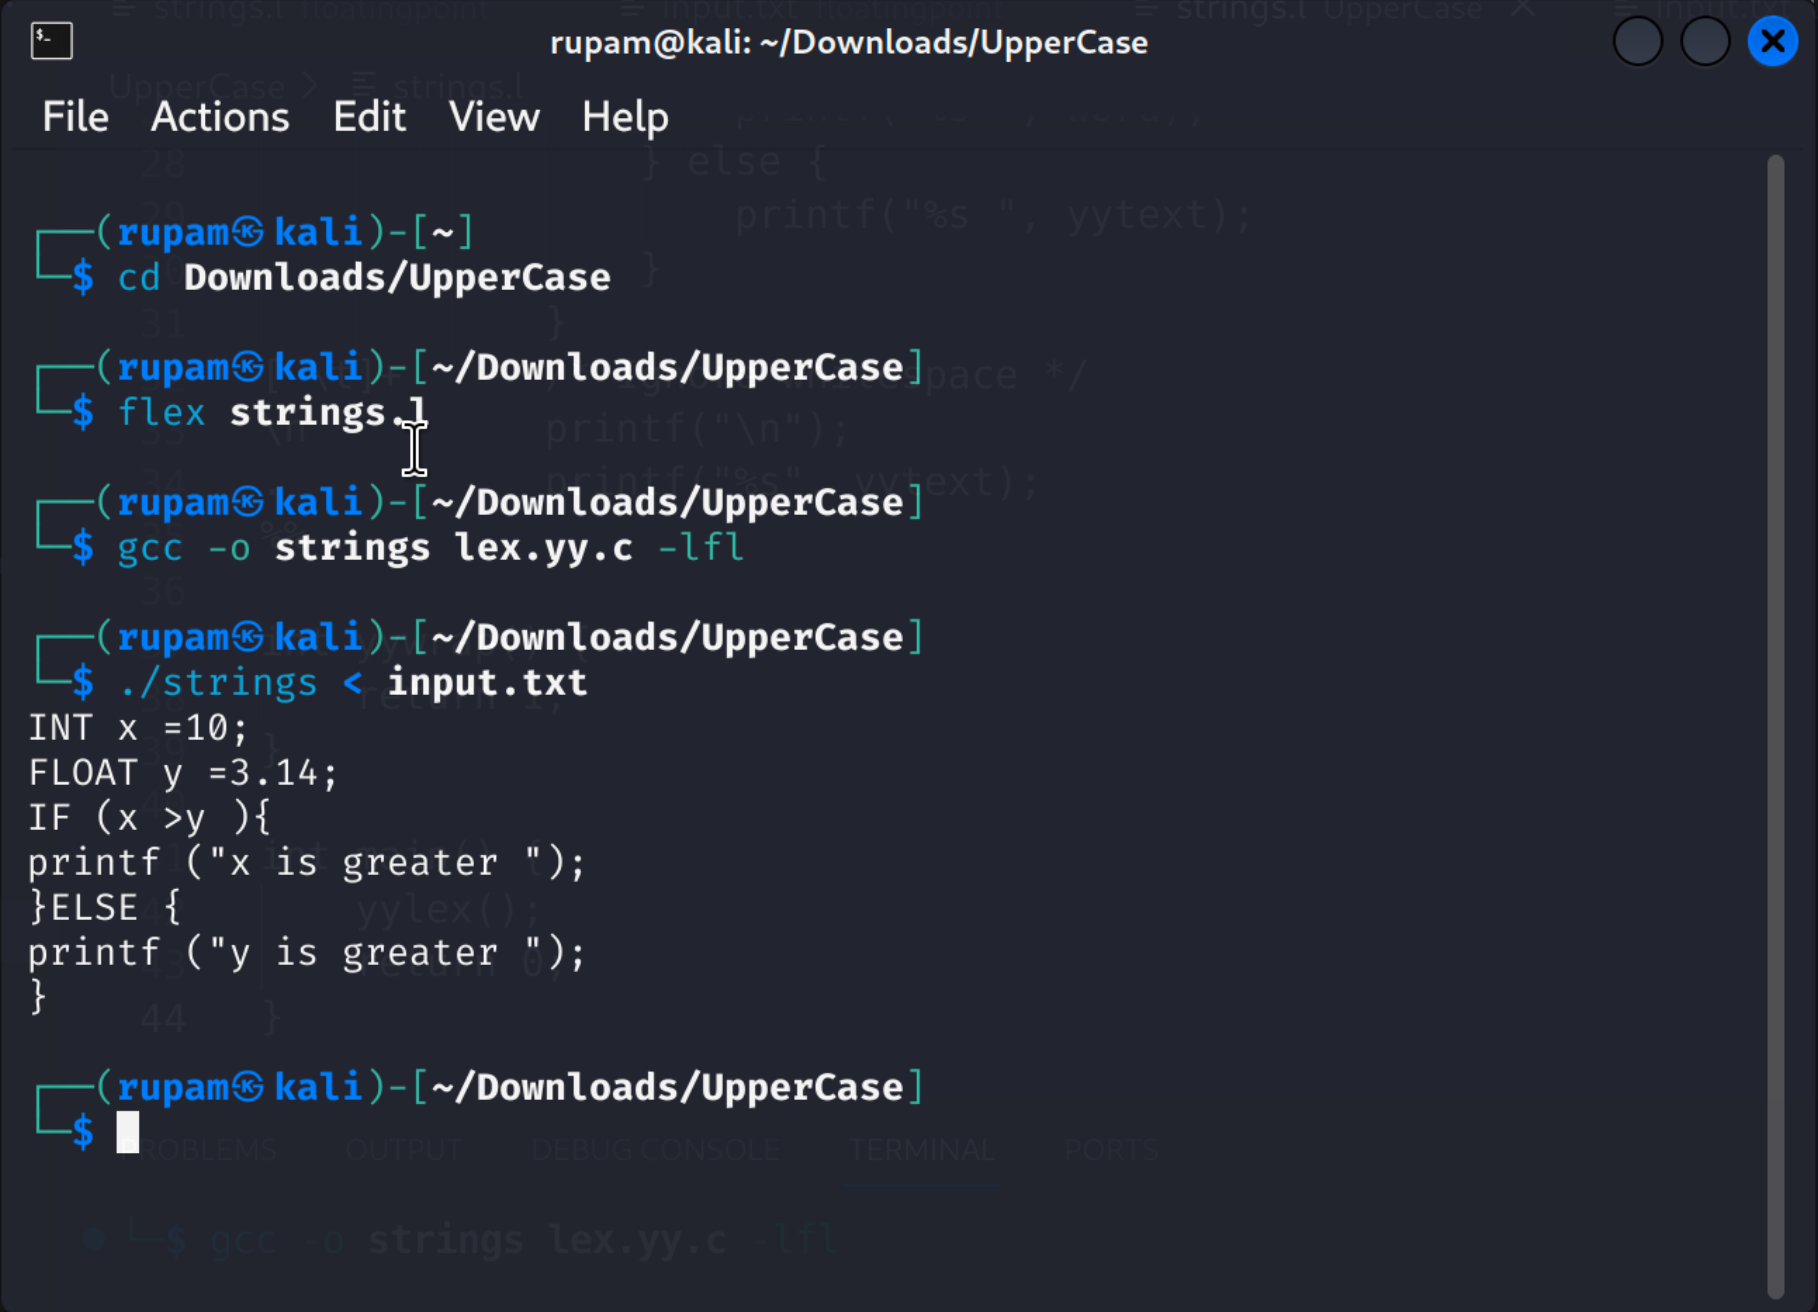
\includegraphics[width=1\linewidth]{exp10output.png}
    \caption{UpperCase Conversion}
\end{figure}

%------------------ EXP 11 Page ------------------
\newpage
\section*{Experiment 11: Lex Program: Count the Number of Vowels and Consonants}
\addcontentsline{toc}{section}{Experiment 11: Lex Program: Count the Number of Vowels and Consonants}

\subsection*{Aim}
\addcontentsline{toc}{subsection}{Aim}
The aim of this experiment is to design and implement a lex program that counts the number of vowels and consonants in the input text.

\subsection*{Objectives}
\addcontentsline{toc}{subsection}{Objectives}
\begin{itemize}
    \item To familiarize with the lex (or flex) utility for lexical analysis tasks related to character classification.
    \item To understand and apply regular expressions for discerning specific categories of characters—namely vowels and consonants.
    \item To create a lex program that categorizes input characters into vowels and consonants and counts their occurrences.
    \item To accurately process input text and ascertain the counts of vowels and consonants, presenting these counts to the user.
    \item To validate the program's correctness and robustness by testing with inputs of varying lengths and compositions.
\end{itemize}

\subsection*{Experiment Code}
\addcontentsline{toc}{subsection}{Experiment Code and Output}
\begin{lstlisting}
%{
  int vowels = 0, consonants = 0;
%}

%%
[aeiouAEIOU]  { vowels++; }
[b-df-hj-np-tv-zB-DF-HJ-NP-TV-Z] { consonants++; }

%%

int main(int argc, char **argv) {
  printf("Enter text (Ctrl+D to end):\n");
  yylex();
  printf("\nNumber of vowels: %d\n", vowels);
  printf("Number of consonants: %d\n", consonants);
  return 0;
}

int yywrap() {
  return 1;
}
\end{lstlisting}
\begin{figure}[H]
    \centering
    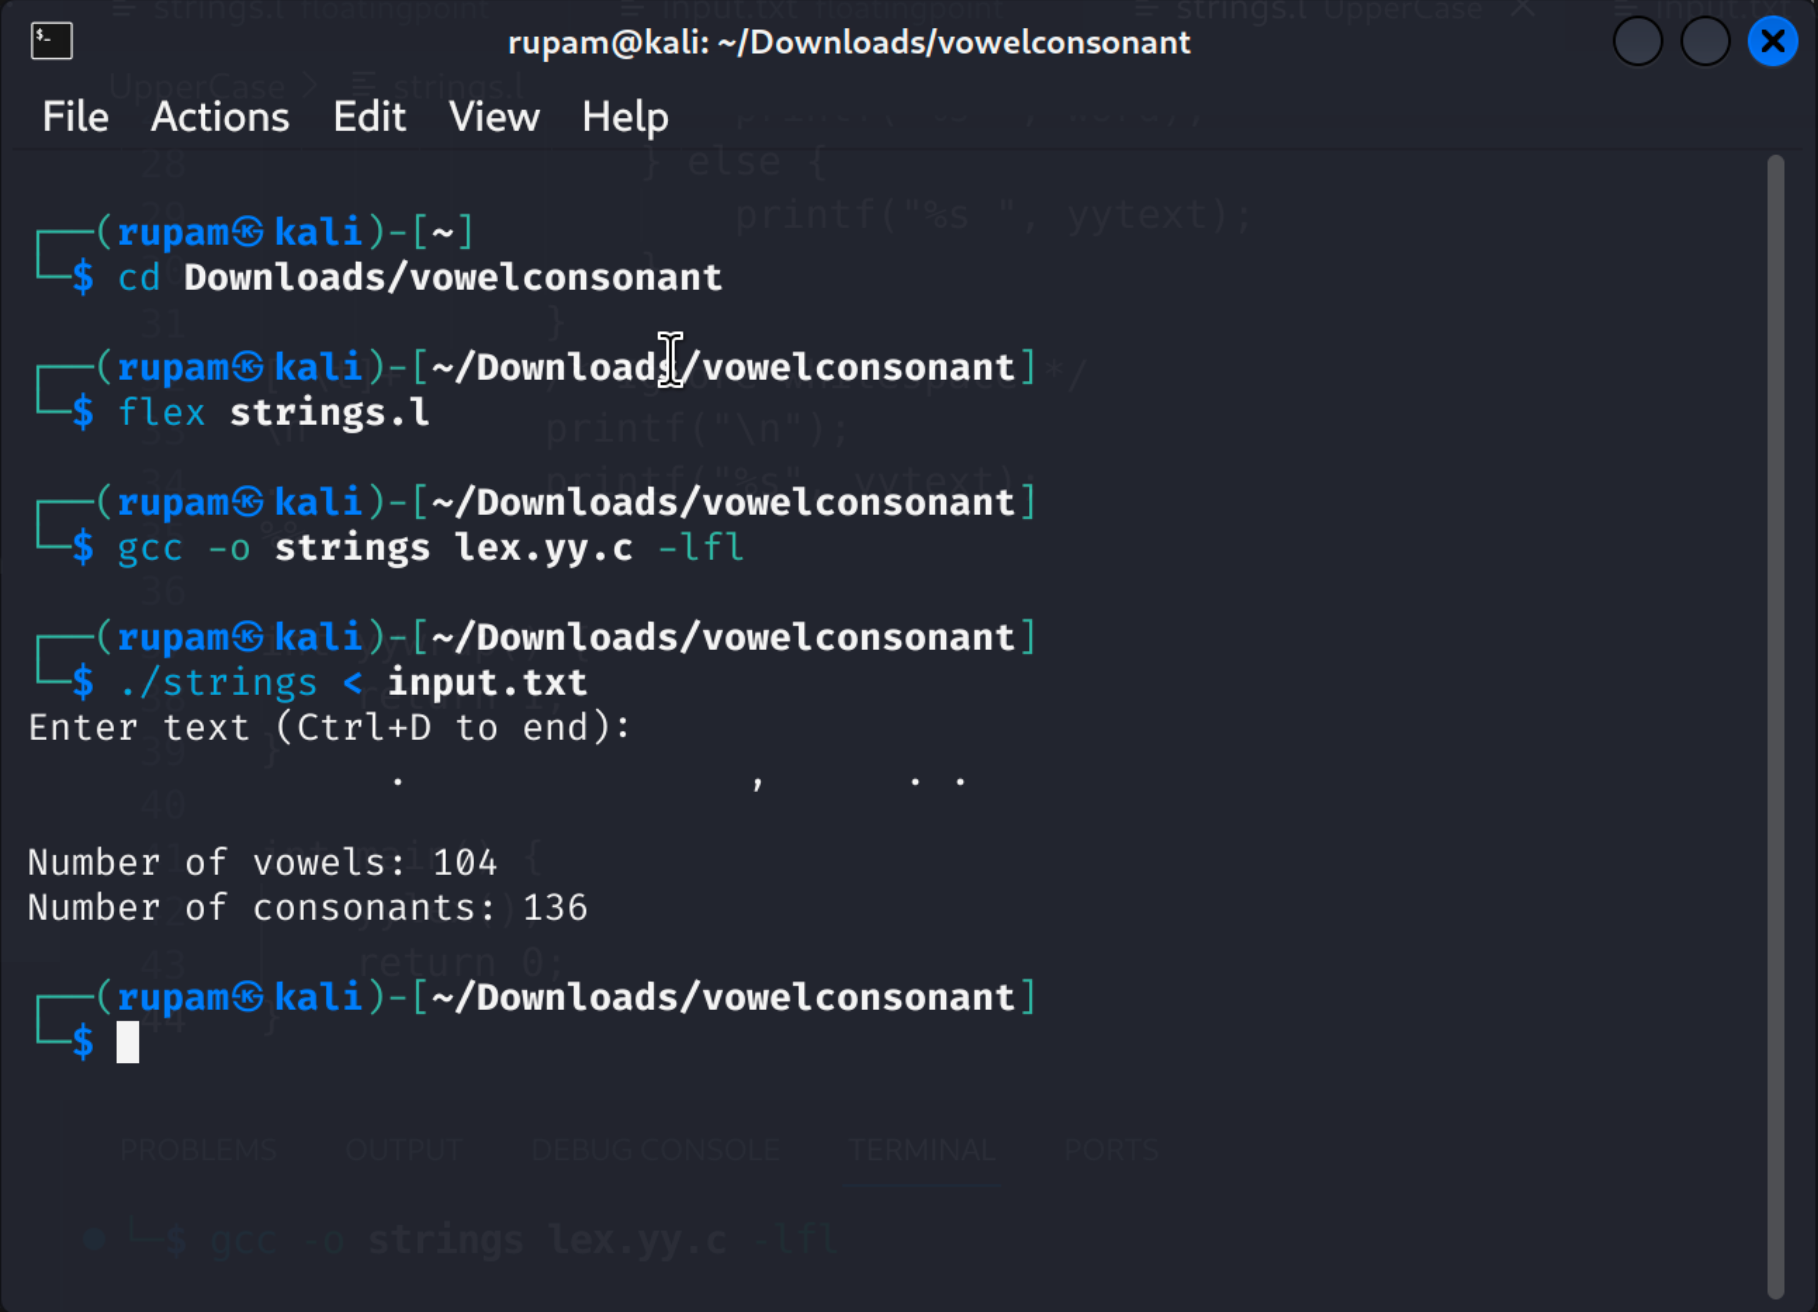
\includegraphics[width=1\linewidth]{exp11output.png}
    \caption{Vowels and Consonants Counter}
\end{figure}

%------------------ EXP 12 Page ------------------
\newpage
\section*{Experiment 12: Lex Program: Count the Number of Identifiers, Keywords, and Digits}
\addcontentsline{toc}{section}{Experiment 12: Lex Program: Count the Number of Identifiers, Keywords, and Digits}

\subsection*{Aim}
\addcontentsline{toc}{subsection}{Aim}
The aim of this experiment is to design and implement a lex program that counts the number of identifiers, keywords, and digit sequences in the provided input text.

\subsection*{Objectives}
\addcontentsline{toc}{subsection}{Objectives}
\begin{itemize}
    \item To deepen understanding of lex (or flex) for lexical analysis involving multiple token types.
    \item To apply regular expression patterns to distinguish between identifiers, keywords, and numeric literals.
    \item To create a lex program that tallies the occurrences of these distinct token types, taking input from text files or standard input.
    \item To ensure the program correctly differentiates between tokens and computes their frequencies.
    \item To assess the program's effectiveness through various test cases encompassing a wide range of inputs.
\end{itemize}

\subsection*{Experiment Code}
\addcontentsline{toc}{subsection}{Experiment Code and Output}
\begin{lstlisting}
%{
  int vowels = 0, consonants = 0;
%}

%%
[aeiouAEIOU]  { vowels++; }
[b-df-hj-np-tv-zB-DF-HJ-NP-TV-Z] { consonants++; }

%%

int main(int argc, char **argv) {
  printf("Enter text (Ctrl+D to end):\n");
  yylex();
  printf("\nNumber of vowels: %d\n", vowels);
  printf("Number of consonants: %d\n", consonants);
  return 0;
}

int yywrap() {
  return 1;
}
\end{lstlisting}
\begin{figure}[H]
    \centering
    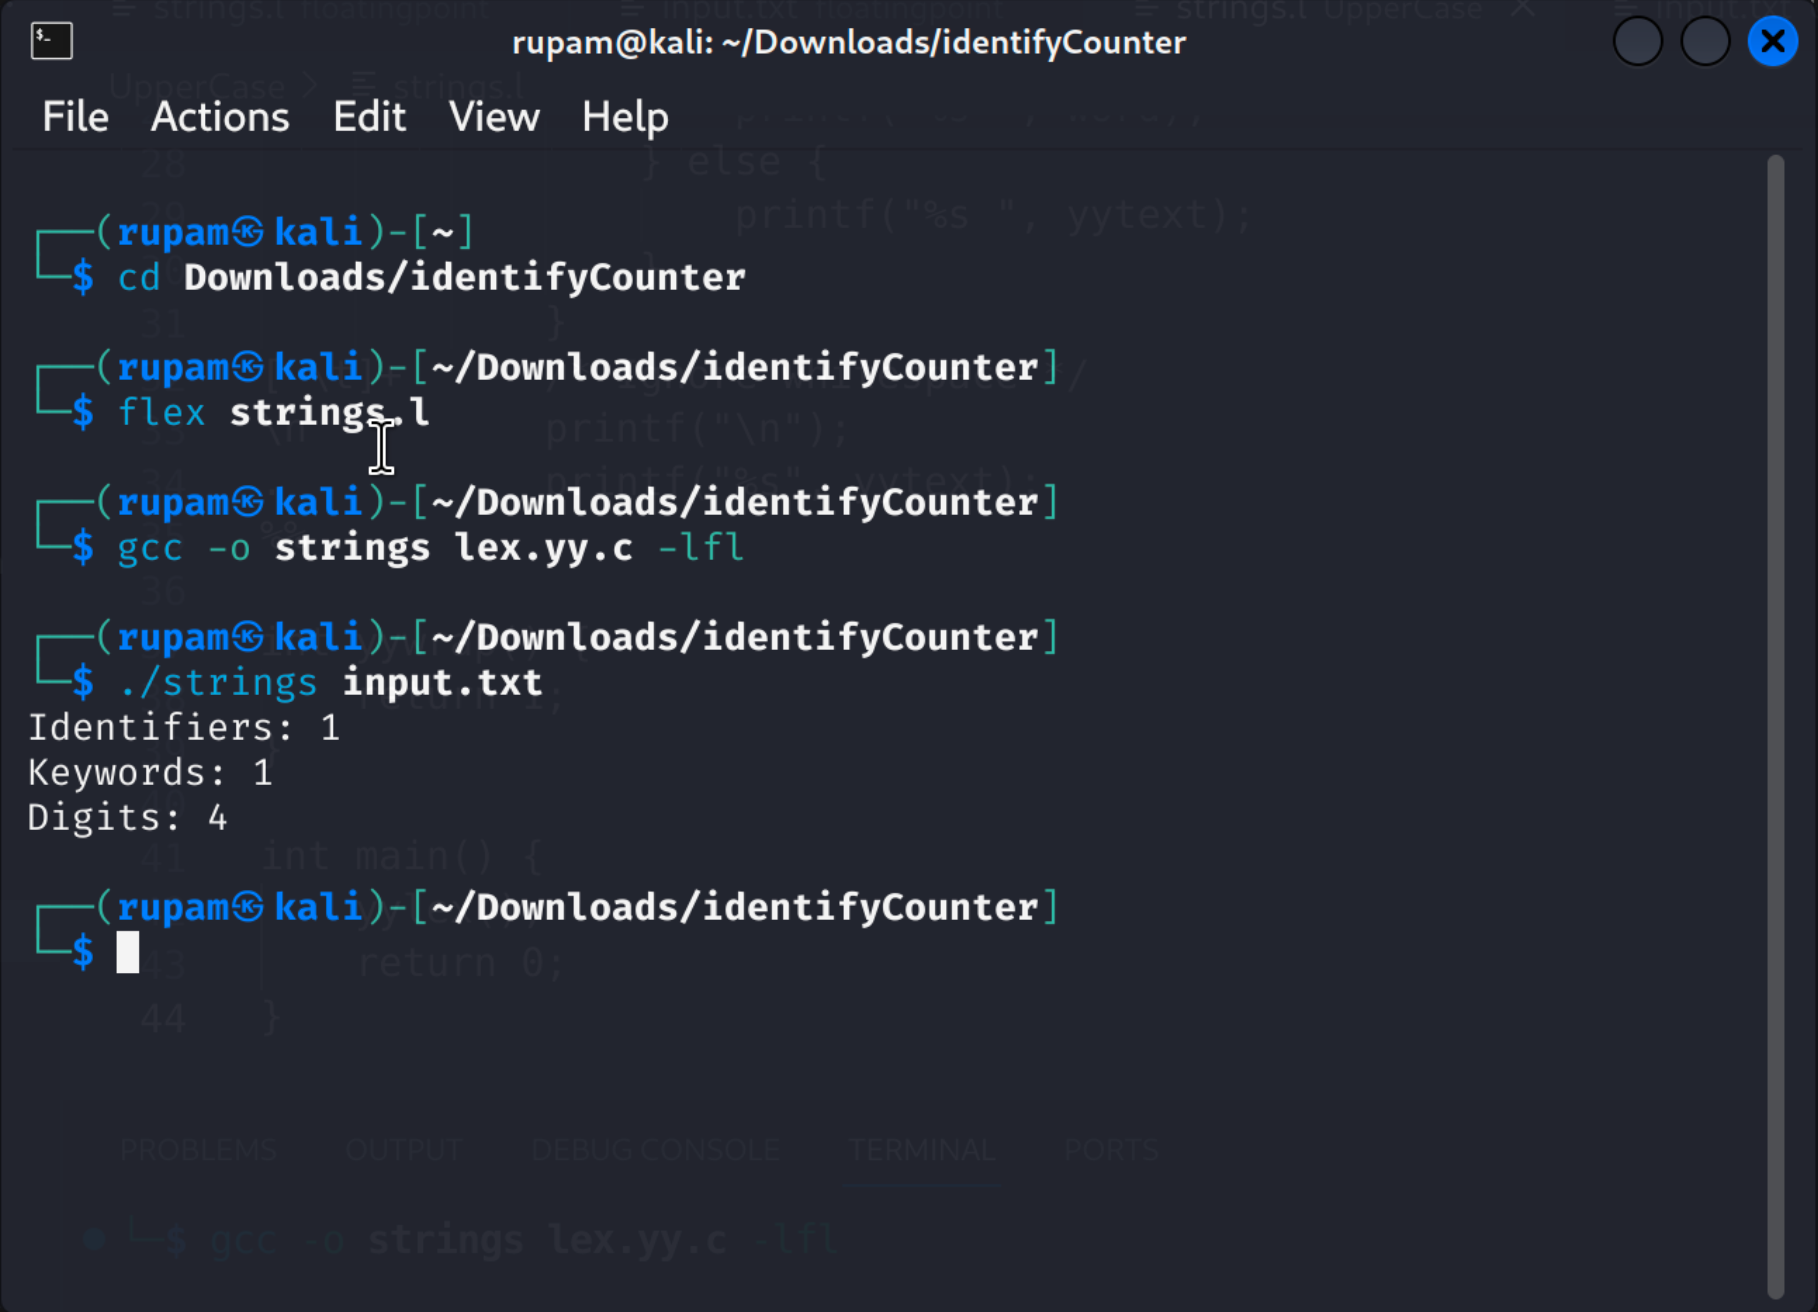
\includegraphics[width=1\linewidth]{exp12output.png}
    \caption{Counter for Identifiers, Keywords, and Digits}
\end{figure}

%------------------ EXP 13 Page ------------------
\newpage
\section*{Experiment 13: Lex Program: Generate all strings over the length seven containing 3 consecutive 2.}
\addcontentsline{toc}{section}{Experiment 13: Lex Program: Generate all strings over the length seven containing 3 consecutive 2.}

\subsection*{Aim}
\addcontentsline{toc}{subsection}{Aim}
The aim of this experiment is to design and implement a lex program to generate strings of length seven that contain a sequence of three consecutive '2's.

\subsection*{Objectives}
\addcontentsline{toc}{subsection}{Objectives}
\begin{itemize}
    \item To investigate and understand the usage of regular expressions within lex (or flex) to define specific string patterns.
    \item To apply knowledge of regular expressions to create a pattern matching rule that identifies strings with three consecutive '2's within seven-character strings.
    \item To develop logic within a lex program to filter strings based on length and specific character repetition criteria.
    \item To ensure the program accurately recognizes strings that match the criteria and rejects others.
    \item To validate the program's capabilities through robust testing with various input combinations.
\end{itemize}

\subsection*{Experiment Code}
\addcontentsline{toc}{subsection}{Experiment Code and Output}
\begin{lstlisting}
%{
#include <stdio.h>
%}
%option noyywrap
%%
%%
int main() {
    // This is not typical usage of Lex.
    // In practice, you would perform this action with a regular C program.
    for (int num = 222; num <= 9999999; num++) {
        // As a string to check with the regex
        char numStr[8];
        sprintf(numStr, "%d", num);
        // Check if "222" is in numStr
        if (strstr(numStr, "222") != NULL) {
            printf("%s\n", numStr);
        }
    }
    return 0;
}
\end{lstlisting}
\begin{figure}[H]
    \centering
    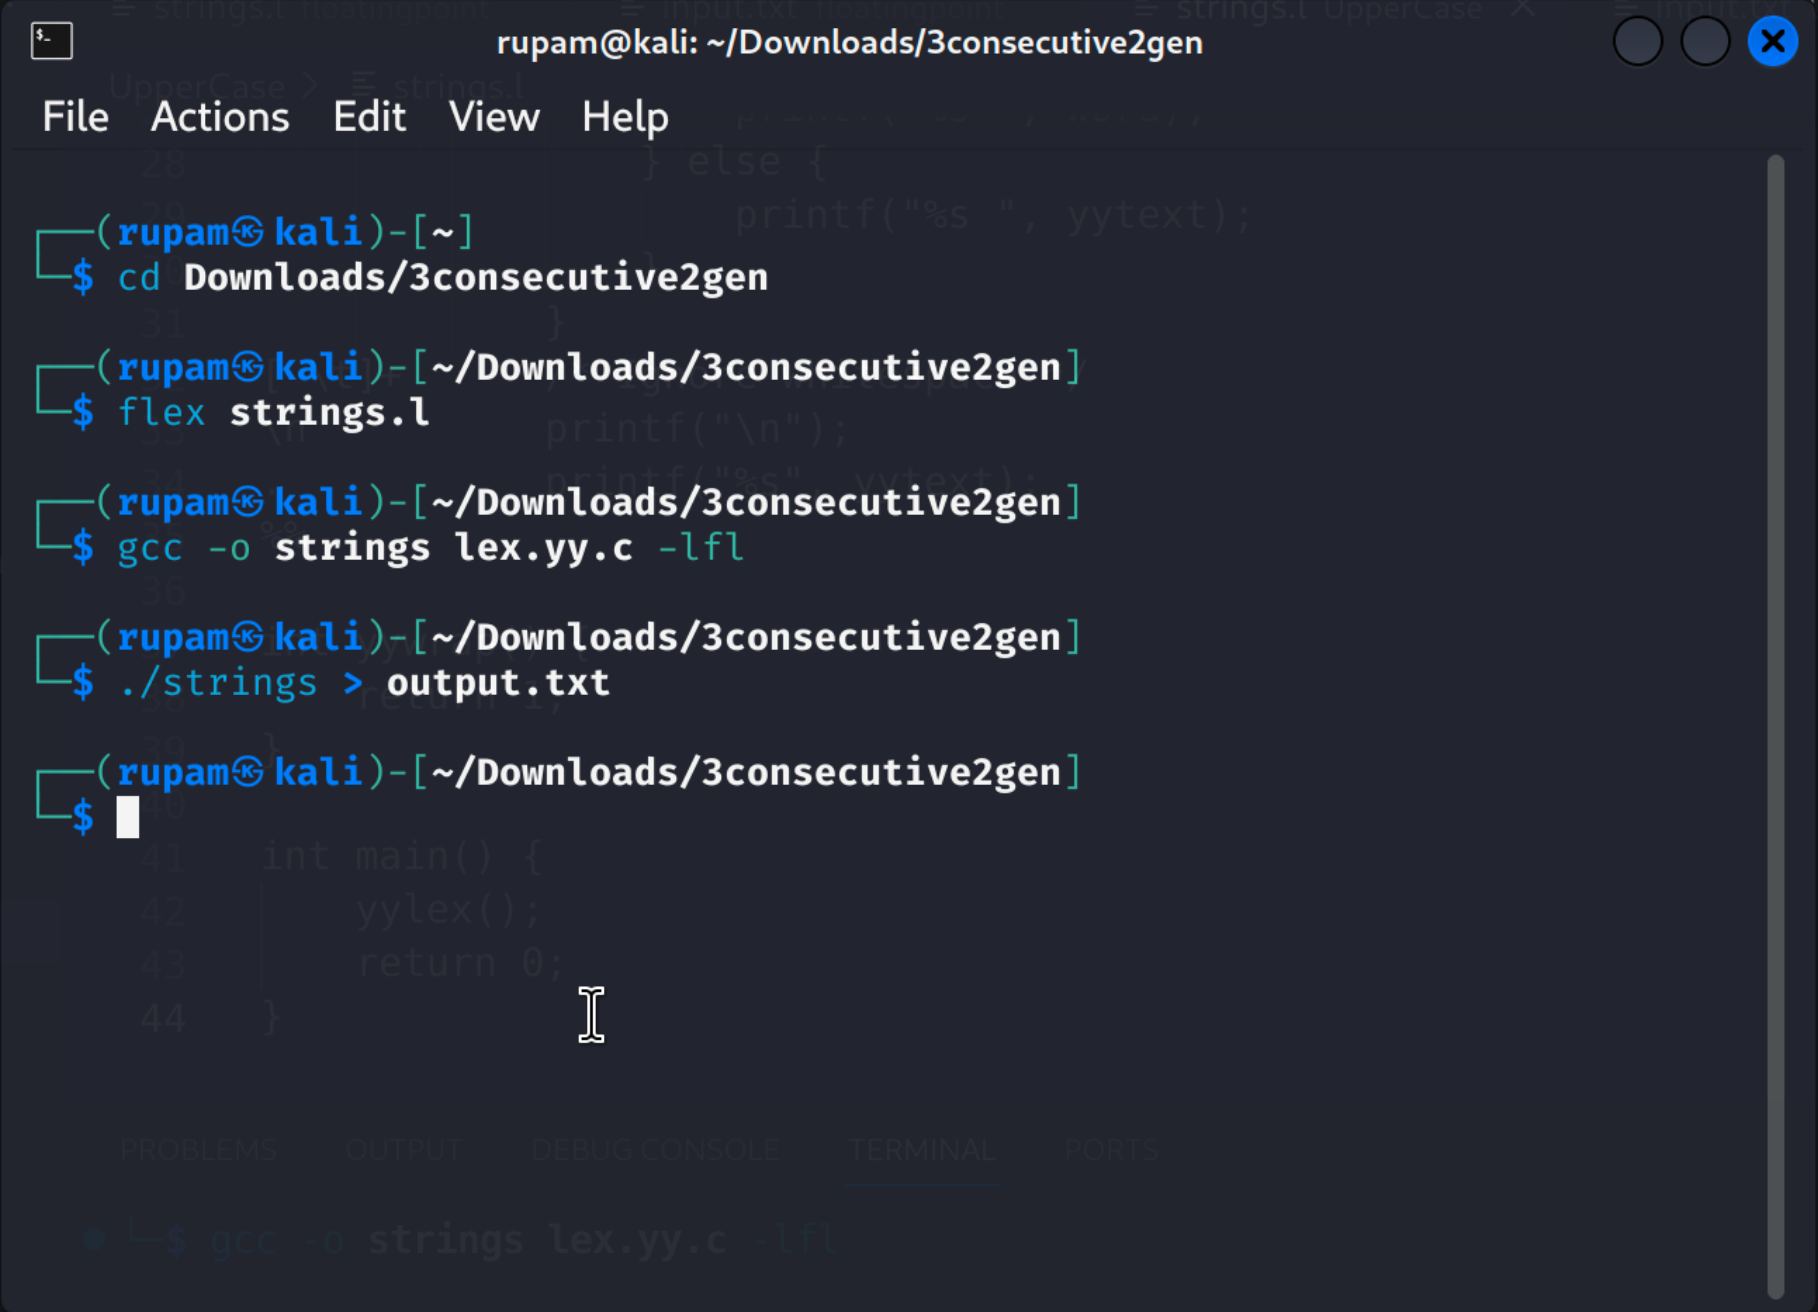
\includegraphics[width=1\linewidth]{exp13command.png}
    \caption{Commands}
\end{figure}
\begin{figure}[H]
    \centering
    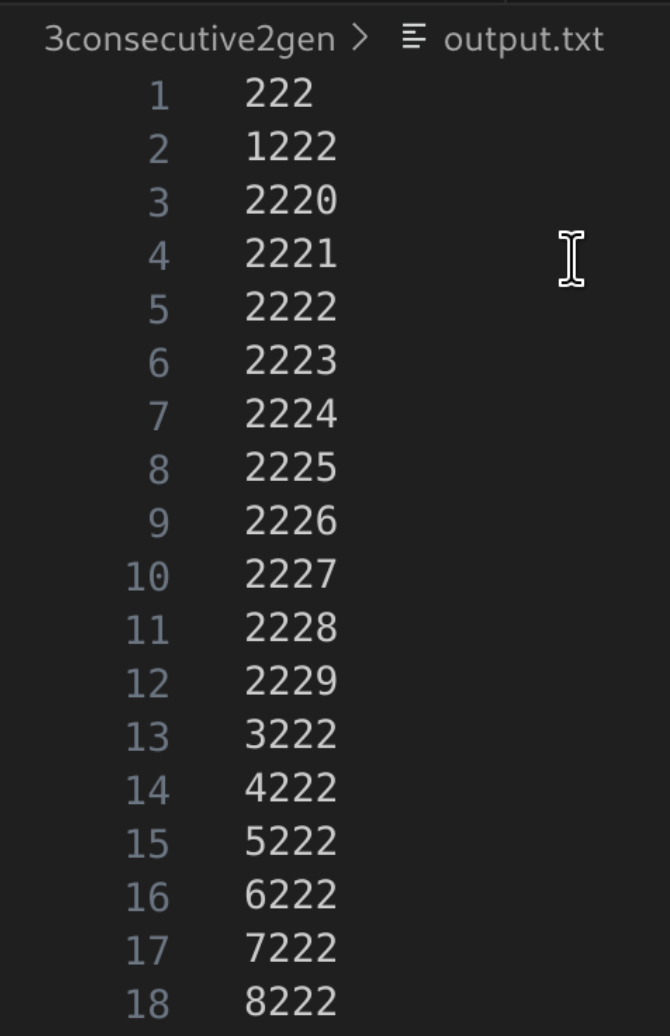
\includegraphics[width=0.5\linewidth]{exp13output.png}
    \caption{Outputs}  
\end{figure}

%------------------ EXP 14 Page ------------------
\newpage
\section*{Experiment 14: Lex Program: Generate all strings over the length five ending with 11.}
\addcontentsline{toc}{section}{Experiment 14: Lex Program: Generate all strings over the length seven ending with 11.}

\subsection*{Aim}
\addcontentsline{toc}{subsection}{Aim}
The aim of this experiment is to design and implement a lex program to generate strings of length seven that end with the string '11'.

\subsection*{Objectives}
\addcontentsline{toc}{subsection}{Objectives}
\begin{itemize}
    \item To understand the construction and utilization of regular expressions for matching strings with specific ending patterns within lex (or flex).
    \item To craft a regular expression pattern that locates strings with a specific suffix, in this case, '11'.
    \item To develop a lex program that identifies and generates strings of exactly five characters in length ending with '11'.
    \item To enable the lex program to process a given list of strings and filter out those that do not fit the specified criteria.
    \item To verify that the lex program accurately identifies the correct strings and ignores those not ending with '11' through comprehensive testing with a range of inputs.
\end{itemize}

\subsection*{Experiment Code}
\addcontentsline{toc}{subsection}{Experiment Code and Output}
\begin{lstlisting}
%option noyywrap
%{
#include <stdio.h>

// Function to generate and print all numbers up to 99999 ending with '11'
void generate_numbers_ending_with_11() {
    for (int i = 0; i < 100000; ++i) {
        if(i % 100 == 11) {
            printf("%05d\n", i);
        }
    }
}
%}
%%
.* ;
%%
int main() {
    generate_numbers_ending_with_11();
    return 0;
}
\end{lstlisting}
\begin{figure}[H]
    \centering
    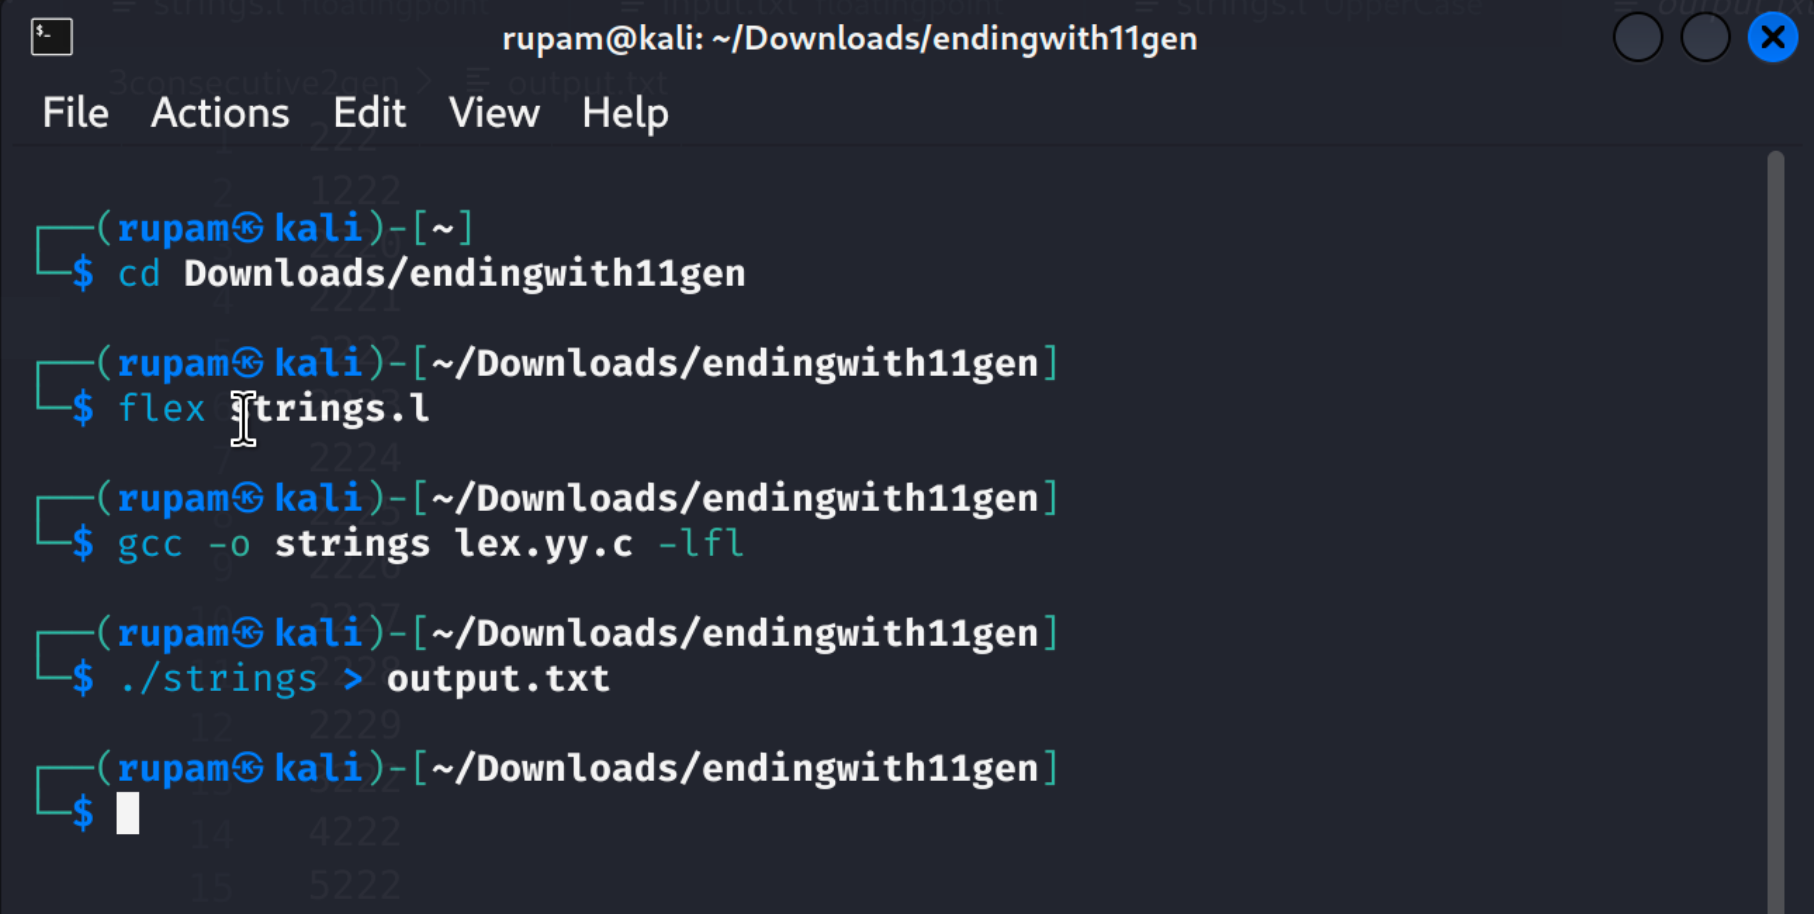
\includegraphics[width=1\linewidth]{exp14command.png}
    \caption{Commands}
\end{figure}
\begin{figure}[H]
    \centering
    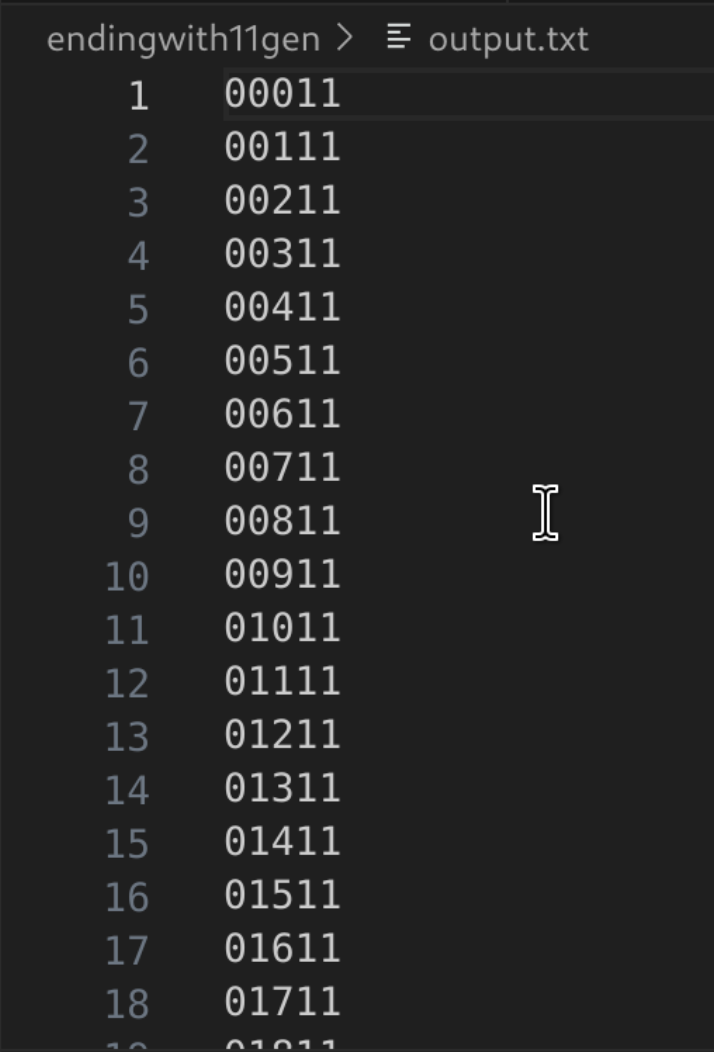
\includegraphics[width=0.5\linewidth]{exp14output.png}
    \caption{Outputs}  
\end{figure}
\end{document}